\documentclass[twoside]{book}

% Packages required by doxygen
\usepackage{fixltx2e}
\usepackage{calc}
\usepackage{doxygen}
\usepackage[export]{adjustbox} % also loads graphicx
\usepackage{graphicx}
\usepackage[utf8]{inputenc}
\usepackage{makeidx}
\usepackage{multicol}
\usepackage{multirow}
\PassOptionsToPackage{warn}{textcomp}
\usepackage{textcomp}
\usepackage[nointegrals]{wasysym}
\usepackage[table]{xcolor}

% Font selection
\usepackage[T1]{fontenc}
\usepackage[scaled=.90]{helvet}
\usepackage{courier}
\usepackage{amssymb}
\usepackage{sectsty}
\renewcommand{\familydefault}{\sfdefault}
\allsectionsfont{%
  \fontseries{bc}\selectfont%
  \color{darkgray}%
}
\renewcommand{\DoxyLabelFont}{%
  \fontseries{bc}\selectfont%
  \color{darkgray}%
}
\newcommand{\+}{\discretionary{\mbox{\scriptsize$\hookleftarrow$}}{}{}}

% Page & text layout
\usepackage{geometry}
\geometry{%
  a4paper,%
  top=2.5cm,%
  bottom=2.5cm,%
  left=2.5cm,%
  right=2.5cm%
}
\tolerance=750
\hfuzz=15pt
\hbadness=750
\setlength{\emergencystretch}{15pt}
\setlength{\parindent}{0cm}
\setlength{\parskip}{3ex plus 2ex minus 2ex}
\makeatletter
\renewcommand{\paragraph}{%
  \@startsection{paragraph}{4}{0ex}{-1.0ex}{1.0ex}{%
    \normalfont\normalsize\bfseries\SS@parafont%
  }%
}
\renewcommand{\subparagraph}{%
  \@startsection{subparagraph}{5}{0ex}{-1.0ex}{1.0ex}{%
    \normalfont\normalsize\bfseries\SS@subparafont%
  }%
}
\makeatother

% Headers & footers
\usepackage{fancyhdr}
\pagestyle{fancyplain}
\fancyhead[LE]{\fancyplain{}{\bfseries\thepage}}
\fancyhead[CE]{\fancyplain{}{}}
\fancyhead[RE]{\fancyplain{}{\bfseries\leftmark}}
\fancyhead[LO]{\fancyplain{}{\bfseries\rightmark}}
\fancyhead[CO]{\fancyplain{}{}}
\fancyhead[RO]{\fancyplain{}{\bfseries\thepage}}
\fancyfoot[LE]{\fancyplain{}{}}
\fancyfoot[CE]{\fancyplain{}{}}
\fancyfoot[RE]{\fancyplain{}{\bfseries\scriptsize Generated by Doxygen }}
\fancyfoot[LO]{\fancyplain{}{\bfseries\scriptsize Generated by Doxygen }}
\fancyfoot[CO]{\fancyplain{}{}}
\fancyfoot[RO]{\fancyplain{}{}}
\renewcommand{\footrulewidth}{0.4pt}
\renewcommand{\chaptermark}[1]{%
  \markboth{#1}{}%
}
\renewcommand{\sectionmark}[1]{%
  \markright{\thesection\ #1}%
}

% Indices & bibliography
\usepackage{natbib}
\usepackage[titles]{tocloft}
\setcounter{tocdepth}{3}
\setcounter{secnumdepth}{5}
\makeindex

% Hyperlinks (required, but should be loaded last)
\usepackage{ifpdf}
\ifpdf
  \usepackage[pdftex,pagebackref=true]{hyperref}
\else
  \usepackage[ps2pdf,pagebackref=true]{hyperref}
\fi
\hypersetup{%
  colorlinks=true,%
  linkcolor=blue,%
  citecolor=blue,%
  unicode%
}

% Custom commands
\newcommand{\clearemptydoublepage}{%
  \newpage{\pagestyle{empty}\cleardoublepage}%
}

\usepackage{caption}
\captionsetup{labelsep=space,justification=centering,font={bf},singlelinecheck=off,skip=4pt,position=top}

%===== C O N T E N T S =====

\begin{document}

% Titlepage & ToC
\hypersetup{pageanchor=false,
             bookmarksnumbered=true,
             pdfencoding=unicode
            }
\pagenumbering{alph}
\begin{titlepage}
\vspace*{7cm}
\begin{center}%
{\Large ascii }\\
\vspace*{1cm}
{\large Generated by Doxygen 1.8.12}\\
\end{center}
\end{titlepage}
\clearemptydoublepage
\pagenumbering{roman}
\tableofcontents
\clearemptydoublepage
\pagenumbering{arabic}
\hypersetup{pageanchor=true}

%--- Begin generated contents ---
\chapter{A\+S\+C\+II P\+R\+O\+J\+E\+CT -\/ C\+O\+U\+RS C++}
\label{index}\hypertarget{index}{}\begin{DoxyAuthor}{Authors}
Whitney Burner 

Raphael Bailly 

Martin Penard
\end{DoxyAuthor}
Jeu A\+S\+C\+II de shoot \textquotesingle{}em up. Pour lancer le jeu, simplement lancer l\textquotesingle{}executable, Pour utiliser le moteur du jeu \+:
\begin{DoxyItemize}
\item Creer les scenes necessaires au jeu
\item Ajouter les scenes au singleton \hyperlink{class_game_engine}{Game\+Engine}
\item Ajouter un (ou des) \hyperlink{class_game_object}{Game\+Object} a une scene \+:
\begin{DoxyItemize}
\item Definir la scene comme scene de debut avec Game\+Engine\+::instance().define\+Starting\+Scene()
\item Ajouter le ou les nouveaux objects au \hyperlink{class_game_engine}{Game\+Engine}
\item Ajouter le ou les scripts (\hyperlink{class_game_component}{Game\+Component}) au \hyperlink{class_game_object}{Game\+Object}
\end{DoxyItemize}
\item Definir la scene par lequel le jeu doit vraiment commencer
\item Appeler Game\+Engine\+::instance().run() 
\end{DoxyItemize}
\chapter{Hierarchical Index}
\section{Class Hierarchy}
This inheritance list is sorted roughly, but not completely, alphabetically\+:\begin{DoxyCompactList}
\item \contentsline{section}{C\+H\+A\+N\+G\+E\+\_\+\+L\+I\+FE}{\pageref{struct_c_h_a_n_g_e___l_i_f_e}}{}
\item \contentsline{section}{Component}{\pageref{class_component}}{}
\begin{DoxyCompactList}
\item \contentsline{section}{Collider\+Component}{\pageref{class_collider_component}}{}
\item \contentsline{section}{Game\+Component}{\pageref{class_game_component}}{}
\begin{DoxyCompactList}
\item \contentsline{section}{Enemy}{\pageref{class_enemy}}{}
\item \contentsline{section}{Game}{\pageref{class_game}}{}
\item \contentsline{section}{Life}{\pageref{class_life}}{}
\item \contentsline{section}{Player}{\pageref{class_player}}{}
\item \contentsline{section}{Rocket}{\pageref{class_rocket}}{}
\item \contentsline{section}{UI}{\pageref{class_u_i}}{}
\item \contentsline{section}{U\+I\+Bullet}{\pageref{class_u_i_bullet}}{}
\end{DoxyCompactList}
\item \contentsline{section}{Graphics\+Component}{\pageref{class_graphics_component}}{}
\item \contentsline{section}{Movement\+Component}{\pageref{class_movement_component}}{}
\item \contentsline{section}{U\+I\+Context\+Component}{\pageref{class_u_i_context_component}}{}
\end{DoxyCompactList}
\item \contentsline{section}{D\+E\+S\+T\+R\+OY}{\pageref{struct_d_e_s_t_r_o_y}}{}
\item \contentsline{section}{Game\+Engine}{\pageref{class_game_engine}}{}
\item \contentsline{section}{Game\+Object}{\pageref{class_game_object}}{}
\item \contentsline{section}{Graphics\+Engine}{\pageref{class_graphics_engine}}{}
\item \contentsline{section}{Input\+Engine}{\pageref{class_input_engine}}{}
\item \contentsline{section}{N\+Y\+Timer}{\pageref{class_n_y_timer}}{}
\item \contentsline{section}{Physics\+Engine}{\pageref{class_physics_engine}}{}
\item \contentsline{section}{Physics\+Ignore}{\pageref{struct_physics_ignore}}{}
\item \contentsline{section}{pixel}{\pageref{structpixel}}{}
\item \contentsline{section}{Scene}{\pageref{class_scene}}{}
\item static\+\_\+visitor\begin{DoxyCompactList}
\item \contentsline{section}{G\+O\+Message\+Handler}{\pageref{class_g_o_message_handler}}{}
\begin{DoxyCompactList}
\item \contentsline{section}{Game\+Component}{\pageref{class_game_component}}{}
\end{DoxyCompactList}
\item \contentsline{section}{S\+C\+Message\+Handler}{\pageref{class_s_c_message_handler}}{}
\end{DoxyCompactList}
\item \contentsline{section}{U\+I\+C\+O\+N\+T\+E\+XT}{\pageref{struct_u_i_c_o_n_t_e_x_t}}{}
\item \contentsline{section}{Vector}{\pageref{class_vector}}{}
\item \contentsline{section}{vector2}{\pageref{structvector2}}{}
\end{DoxyCompactList}

\chapter{Class Index}
\section{Class List}
Here are the classes, structs, unions and interfaces with brief descriptions\+:\begin{DoxyCompactList}
\item\contentsline{section}{\hyperlink{struct_c_h_a_n_g_e___l_i_f_e}{C\+H\+A\+N\+G\+E\+\_\+\+L\+I\+FE} }{\pageref{struct_c_h_a_n_g_e___l_i_f_e}}{}
\item\contentsline{section}{\hyperlink{class_collider_component}{Collider\+Component} \\*\hyperlink{class_component}{Component} contenant la hitbox du \hyperlink{class_game_object}{Game\+Object} qui le contient }{\pageref{class_collider_component}}{}
\item\contentsline{section}{\hyperlink{class_component}{Component} \\*Interface de \hyperlink{class_component}{Component} }{\pageref{class_component}}{}
\item\contentsline{section}{\hyperlink{struct_d_e_s_t_r_o_y}{D\+E\+S\+T\+R\+OY} }{\pageref{struct_d_e_s_t_r_o_y}}{}
\item\contentsline{section}{\hyperlink{class_enemy}{Enemy} }{\pageref{class_enemy}}{}
\item\contentsline{section}{\hyperlink{class_game}{Game} }{\pageref{class_game}}{}
\item\contentsline{section}{\hyperlink{class_game_component}{Game\+Component} \\*Classe de base des scripts utilisateurs }{\pageref{class_game_component}}{}
\item\contentsline{section}{\hyperlink{class_game_engine}{Game\+Engine} \\*Classe Singleton prenant en charge les \hyperlink{class_scene}{Scene} et la boucle de jeu }{\pageref{class_game_engine}}{}
\item\contentsline{section}{\hyperlink{class_game_object}{Game\+Object} }{\pageref{class_game_object}}{}
\item\contentsline{section}{\hyperlink{class_g_o_message_handler}{G\+O\+Message\+Handler} \\*Message recu et envoyer par les \hyperlink{class_game_object}{Game\+Object}, qui les dispatchent aux Game\+Components }{\pageref{class_g_o_message_handler}}{}
\item\contentsline{section}{\hyperlink{class_graphics_component}{Graphics\+Component} \\*\hyperlink{class_component}{Component} contenant un sprite a afficher dans la console }{\pageref{class_graphics_component}}{}
\item\contentsline{section}{\hyperlink{class_graphics_engine}{Graphics\+Engine} \\*Classe permettant l\textquotesingle{}affichage du jeu }{\pageref{class_graphics_engine}}{}
\item\contentsline{section}{\hyperlink{class_input_engine}{Input\+Engine} \\*Classe prenant en charge la gestion des inputs utilisateur }{\pageref{class_input_engine}}{}
\item\contentsline{section}{\hyperlink{class_life}{Life} \\*Script gerant le vie d\textquotesingle{}un gameobject }{\pageref{class_life}}{}
\item\contentsline{section}{\hyperlink{class_movement_component}{Movement\+Component} \\*\hyperlink{class_component}{Component} une velocite }{\pageref{class_movement_component}}{}
\item\contentsline{section}{\hyperlink{class_n_y_timer}{N\+Y\+Timer} }{\pageref{class_n_y_timer}}{}
\item\contentsline{section}{\hyperlink{class_physics_engine}{Physics\+Engine} \\*Classe prenant en charge la gestion de la physique du jeu }{\pageref{class_physics_engine}}{}
\item\contentsline{section}{\hyperlink{struct_physics_ignore}{Physics\+Ignore} }{\pageref{struct_physics_ignore}}{}
\item\contentsline{section}{\hyperlink{structpixel}{pixel} }{\pageref{structpixel}}{}
\item\contentsline{section}{\hyperlink{class_player}{Player} }{\pageref{class_player}}{}
\item\contentsline{section}{\hyperlink{class_rocket}{Rocket} }{\pageref{class_rocket}}{}
\item\contentsline{section}{\hyperlink{class_scene}{Scene} \\*Classe gerant une scene, c\textquotesingle{}est a dire une liste de \hyperlink{class_game_object}{Game\+Object} }{\pageref{class_scene}}{}
\item\contentsline{section}{\hyperlink{class_s_c_message_handler}{S\+C\+Message\+Handler} }{\pageref{class_s_c_message_handler}}{}
\item\contentsline{section}{\hyperlink{class_u_i}{UI} }{\pageref{class_u_i}}{}
\item\contentsline{section}{\hyperlink{class_u_i_bullet}{U\+I\+Bullet} }{\pageref{class_u_i_bullet}}{}
\item\contentsline{section}{\hyperlink{struct_u_i_c_o_n_t_e_x_t}{U\+I\+C\+O\+N\+T\+E\+XT} }{\pageref{struct_u_i_c_o_n_t_e_x_t}}{}
\item\contentsline{section}{\hyperlink{structvector2}{vector2} }{\pageref{structvector2}}{}
\end{DoxyCompactList}

\chapter{Class Documentation}
\hypertarget{struct_c_h_a_n_g_e___l_i_f_e}{}\section{C\+H\+A\+N\+G\+E\+\_\+\+L\+I\+FE Struct Reference}
\label{struct_c_h_a_n_g_e___l_i_f_e}\index{C\+H\+A\+N\+G\+E\+\_\+\+L\+I\+FE@{C\+H\+A\+N\+G\+E\+\_\+\+L\+I\+FE}}
\subsection*{Public Attributes}
\begin{DoxyCompactItemize}
\item 
\hypertarget{struct_c_h_a_n_g_e___l_i_f_e_a280cc46bec0a074b57444849f2faebf0}{}\label{struct_c_h_a_n_g_e___l_i_f_e_a280cc46bec0a074b57444849f2faebf0} 
int {\bfseries value}
\end{DoxyCompactItemize}


The documentation for this struct was generated from the following file\+:\begin{DoxyCompactItemize}
\item 
F\+:/\+\_\+\+\_\+\+M\+A\+R\+T\+I\+N/\+\_\+\+\_\+\+E\+N\+J\+M\+I\+N/\+Projets/ascii/shooter/\+A\+S\+C\+I\+I\+\_\+\+S\+H\+O\+O\+T\+E\+R\+\_\+\+P\+R\+O\+T\+O/Message\+Handler.\+h\end{DoxyCompactItemize}

\hypertarget{class_collider_component}{}\section{Collider\+Component Class Reference}
\label{class_collider_component}\index{Collider\+Component@{Collider\+Component}}


\hyperlink{class_component}{Component} contenant la hitbox du \hyperlink{class_game_object}{Game\+Object} qui le contient.  




{\ttfamily \#include $<$Collider\+Component.\+h$>$}

Inheritance diagram for Collider\+Component\+:\begin{figure}[H]
\begin{center}
\leavevmode
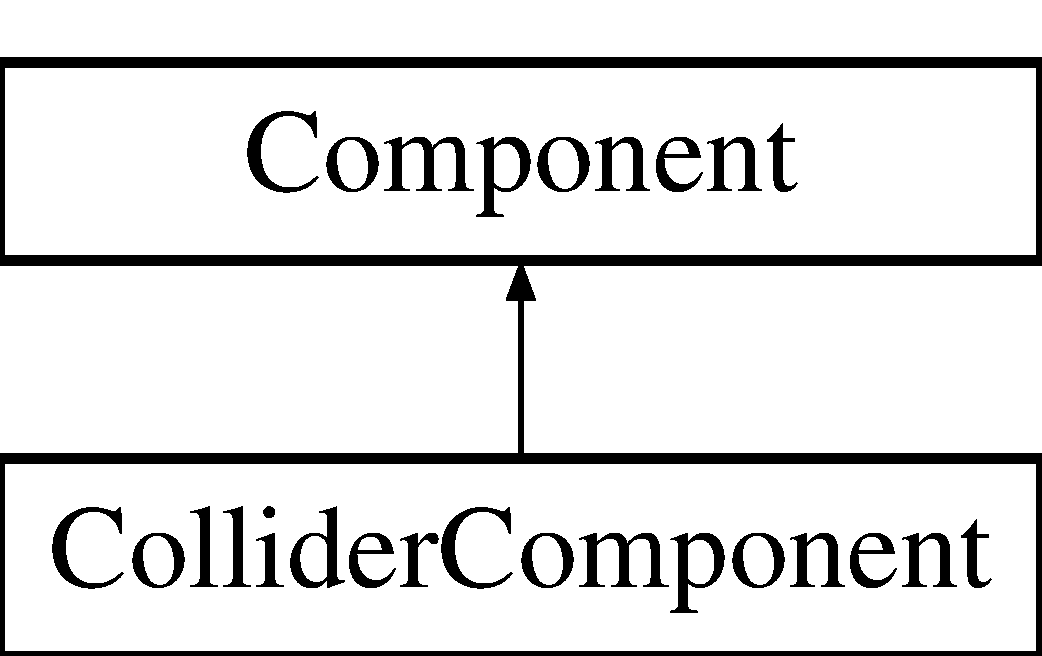
\includegraphics[height=2.000000cm]{class_collider_component}
\end{center}
\end{figure}
\subsection*{Public Member Functions}
\begin{DoxyCompactItemize}
\item 
\hypertarget{class_collider_component_ac83b2680f1a5fc244ef2708e86575fa4}{}\label{class_collider_component_ac83b2680f1a5fc244ef2708e86575fa4} 
\hyperlink{class_collider_component_ac83b2680f1a5fc244ef2708e86575fa4}{Collider\+Component} (\hyperlink{class_game_object}{Game\+Object} $\ast$obj)
\begin{DoxyCompactList}\small\item\em Creer un Collider de base de taille (0,0) \end{DoxyCompactList}\item 
\hyperlink{class_collider_component_a6a7e494fa3fea02a82d0c73f3f862818}{Collider\+Component} (\hyperlink{class_game_object}{Game\+Object} $\ast$obj, float x, float y)
\begin{DoxyCompactList}\small\item\em Creer un Collider de taille (x,y) \end{DoxyCompactList}\item 
\hyperlink{class_collider_component_a5d8271253d38e57635235d0d5b083561}{Collider\+Component} (\hyperlink{class_game_object}{Game\+Object} $\ast$obj, \hyperlink{structvector2}{vector2} hitbox)
\begin{DoxyCompactList}\small\item\em Creer un Collider a partir d\textquotesingle{}un \hyperlink{structvector2}{vector2}. \end{DoxyCompactList}\item 
void \hyperlink{class_collider_component_ac745e518856d98ae5f0d53b356c390f7}{set\+Hit\+Box} (const \hyperlink{structvector2}{vector2} \&hb)
\begin{DoxyCompactList}\small\item\em Setter de la hitbox par copie. \end{DoxyCompactList}\item 
void \hyperlink{class_collider_component_a21bf46d6f8049e2832e07a896a91f7b0}{set\+Hit\+Box} (const float x, const float y)
\begin{DoxyCompactList}\small\item\em Setter de la hitbox a partir de 2 float. \end{DoxyCompactList}\item 
\hyperlink{structvector2}{vector2} \& \hyperlink{class_collider_component_ad0c16141d83ab4d8c249d8f61355f691}{get\+Hit\+Box} ()
\begin{DoxyCompactList}\small\item\em Getter de la hitbox. \end{DoxyCompactList}\end{DoxyCompactItemize}
\subsection*{Protected Attributes}
\begin{DoxyCompactItemize}
\item 
\hypertarget{class_collider_component_a9d1e72e0e45b58f19d644aae2fd2ee4c}{}\label{class_collider_component_a9d1e72e0e45b58f19d644aae2fd2ee4c} 
\hyperlink{structvector2}{vector2} {\bfseries \+\_\+hitbox}
\end{DoxyCompactItemize}


\subsection{Detailed Description}
\hyperlink{class_component}{Component} contenant la hitbox du \hyperlink{class_game_object}{Game\+Object} qui le contient. 

\subsection{Constructor \& Destructor Documentation}
\hypertarget{class_collider_component_a6a7e494fa3fea02a82d0c73f3f862818}{}\label{class_collider_component_a6a7e494fa3fea02a82d0c73f3f862818} 
\index{Collider\+Component@{Collider\+Component}!Collider\+Component@{Collider\+Component}}
\index{Collider\+Component@{Collider\+Component}!Collider\+Component@{Collider\+Component}}
\subsubsection{\texorpdfstring{Collider\+Component()}{ColliderComponent()}\hspace{0.1cm}{\footnotesize\ttfamily [1/2]}}
{\footnotesize\ttfamily Collider\+Component\+::\+Collider\+Component (\begin{DoxyParamCaption}\item[{\hyperlink{class_game_object}{Game\+Object} $\ast$}]{obj,  }\item[{float}]{x,  }\item[{float}]{y }\end{DoxyParamCaption})\hspace{0.3cm}{\ttfamily [inline]}}



Creer un Collider de taille (x,y) 


\begin{DoxyParams}{Parameters}
{\em x} & \+: taille x de la hitbox \\
\hline
{\em y} & \+: taille y de la hitbox \\
\hline
\end{DoxyParams}
\hypertarget{class_collider_component_a5d8271253d38e57635235d0d5b083561}{}\label{class_collider_component_a5d8271253d38e57635235d0d5b083561} 
\index{Collider\+Component@{Collider\+Component}!Collider\+Component@{Collider\+Component}}
\index{Collider\+Component@{Collider\+Component}!Collider\+Component@{Collider\+Component}}
\subsubsection{\texorpdfstring{Collider\+Component()}{ColliderComponent()}\hspace{0.1cm}{\footnotesize\ttfamily [2/2]}}
{\footnotesize\ttfamily Collider\+Component\+::\+Collider\+Component (\begin{DoxyParamCaption}\item[{\hyperlink{class_game_object}{Game\+Object} $\ast$}]{obj,  }\item[{\hyperlink{structvector2}{vector2}}]{hitbox }\end{DoxyParamCaption})\hspace{0.3cm}{\ttfamily [inline]}}



Creer un Collider a partir d\textquotesingle{}un \hyperlink{structvector2}{vector2}. 


\begin{DoxyParams}{Parameters}
{\em \hyperlink{structvector2}{vector2}} & qui sera copie dans la hitbox du Collider \\
\hline
\end{DoxyParams}


\subsection{Member Function Documentation}
\hypertarget{class_collider_component_ad0c16141d83ab4d8c249d8f61355f691}{}\label{class_collider_component_ad0c16141d83ab4d8c249d8f61355f691} 
\index{Collider\+Component@{Collider\+Component}!get\+Hit\+Box@{get\+Hit\+Box}}
\index{get\+Hit\+Box@{get\+Hit\+Box}!Collider\+Component@{Collider\+Component}}
\subsubsection{\texorpdfstring{get\+Hit\+Box()}{getHitBox()}}
{\footnotesize\ttfamily \hyperlink{structvector2}{vector2}\& Collider\+Component\+::get\+Hit\+Box (\begin{DoxyParamCaption}{ }\end{DoxyParamCaption})\hspace{0.3cm}{\ttfamily [inline]}}



Getter de la hitbox. 

\begin{DoxyReturn}{Returns}
une r�f�rence la hitbox 
\end{DoxyReturn}
\hypertarget{class_collider_component_ac745e518856d98ae5f0d53b356c390f7}{}\label{class_collider_component_ac745e518856d98ae5f0d53b356c390f7} 
\index{Collider\+Component@{Collider\+Component}!set\+Hit\+Box@{set\+Hit\+Box}}
\index{set\+Hit\+Box@{set\+Hit\+Box}!Collider\+Component@{Collider\+Component}}
\subsubsection{\texorpdfstring{set\+Hit\+Box()}{setHitBox()}\hspace{0.1cm}{\footnotesize\ttfamily [1/2]}}
{\footnotesize\ttfamily void Collider\+Component\+::set\+Hit\+Box (\begin{DoxyParamCaption}\item[{const \hyperlink{structvector2}{vector2} \&}]{hb }\end{DoxyParamCaption})\hspace{0.3cm}{\ttfamily [inline]}}



Setter de la hitbox par copie. 


\begin{DoxyParams}{Parameters}
{\em la} & hitbox a copier \\
\hline
\end{DoxyParams}
\hypertarget{class_collider_component_a21bf46d6f8049e2832e07a896a91f7b0}{}\label{class_collider_component_a21bf46d6f8049e2832e07a896a91f7b0} 
\index{Collider\+Component@{Collider\+Component}!set\+Hit\+Box@{set\+Hit\+Box}}
\index{set\+Hit\+Box@{set\+Hit\+Box}!Collider\+Component@{Collider\+Component}}
\subsubsection{\texorpdfstring{set\+Hit\+Box()}{setHitBox()}\hspace{0.1cm}{\footnotesize\ttfamily [2/2]}}
{\footnotesize\ttfamily void Collider\+Component\+::set\+Hit\+Box (\begin{DoxyParamCaption}\item[{const float}]{x,  }\item[{const float}]{y }\end{DoxyParamCaption})\hspace{0.3cm}{\ttfamily [inline]}}



Setter de la hitbox a partir de 2 float. 


\begin{DoxyParams}{Parameters}
{\em valeurs} & x et y de la hitbox \\
\hline
\end{DoxyParams}


The documentation for this class was generated from the following file\+:\begin{DoxyCompactItemize}
\item 
F\+:/\+\_\+\+\_\+\+M\+A\+R\+T\+I\+N/\+\_\+\+\_\+\+E\+N\+J\+M\+I\+N/\+Projets/ascii/shooter/\+A\+S\+C\+I\+I\+\_\+\+S\+H\+O\+O\+T\+E\+R\+\_\+\+P\+R\+O\+T\+O/Collider\+Component.\+h\end{DoxyCompactItemize}

\hypertarget{class_component}{}\section{Component Class Reference}
\label{class_component}\index{Component@{Component}}


Interface de \hyperlink{class_component}{Component}.  




{\ttfamily \#include $<$Component.\+h$>$}

Inheritance diagram for Component\+:\begin{figure}[H]
\begin{center}
\leavevmode
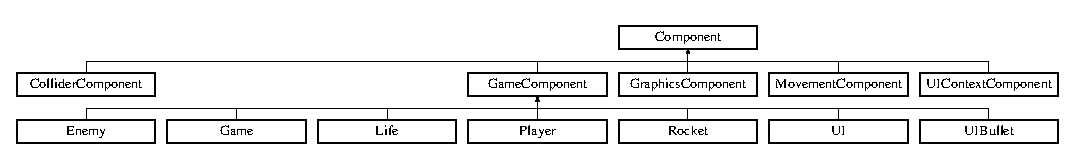
\includegraphics[height=1.702128cm]{class_component}
\end{center}
\end{figure}
\subsection*{Public Member Functions}
\begin{DoxyCompactItemize}
\item 
\hypertarget{class_component_a3d2ef69dcd0e27152de94fc7bb4f01de}{}\label{class_component_a3d2ef69dcd0e27152de94fc7bb4f01de} 
{\bfseries Component} (\hyperlink{class_game_object}{Game\+Object} $\ast$)
\item 
\hypertarget{class_component_a9c76099b7507595bc7f2eeecec3f9828}{}\label{class_component_a9c76099b7507595bc7f2eeecec3f9828} 
\hyperlink{class_game_object}{Game\+Object} $\ast$ {\bfseries get\+Game\+Object} ()
\end{DoxyCompactItemize}
\subsection*{Protected Attributes}
\begin{DoxyCompactItemize}
\item 
\hypertarget{class_component_ac52c4a811c3f8b64f3cd3306da81fba5}{}\label{class_component_ac52c4a811c3f8b64f3cd3306da81fba5} 
\hyperlink{class_game_object}{Game\+Object} $\ast$ {\bfseries \+\_\+game\+Object}
\end{DoxyCompactItemize}


\subsection{Detailed Description}
Interface de \hyperlink{class_component}{Component}. 

The documentation for this class was generated from the following files\+:\begin{DoxyCompactItemize}
\item 
F\+:/\+\_\+\+\_\+\+M\+A\+R\+T\+I\+N/\+\_\+\+\_\+\+E\+N\+J\+M\+I\+N/\+Projets/ascii/shooter/\+A\+S\+C\+I\+I\+\_\+\+S\+H\+O\+O\+T\+E\+R\+\_\+\+P\+R\+O\+T\+O/Component.\+h\item 
F\+:/\+\_\+\+\_\+\+M\+A\+R\+T\+I\+N/\+\_\+\+\_\+\+E\+N\+J\+M\+I\+N/\+Projets/ascii/shooter/\+A\+S\+C\+I\+I\+\_\+\+S\+H\+O\+O\+T\+E\+R\+\_\+\+P\+R\+O\+T\+O/Component.\+cpp\end{DoxyCompactItemize}

\hypertarget{struct_d_e_s_t_r_o_y}{}\section{D\+E\+S\+T\+R\+OY Struct Reference}
\label{struct_d_e_s_t_r_o_y}\index{D\+E\+S\+T\+R\+OY@{D\+E\+S\+T\+R\+OY}}


The documentation for this struct was generated from the following file\+:\begin{DoxyCompactItemize}
\item 
F\+:/\+\_\+\+\_\+\+M\+A\+R\+T\+I\+N/\+\_\+\+\_\+\+E\+N\+J\+M\+I\+N/\+Projets/ascii/shooter/\+A\+S\+C\+I\+I\+\_\+\+S\+H\+O\+O\+T\+E\+R\+\_\+\+P\+R\+O\+T\+O/Message\+Handler.\+h\end{DoxyCompactItemize}

\hypertarget{class_enemy}{}\section{Enemy Class Reference}
\label{class_enemy}\index{Enemy@{Enemy}}
Inheritance diagram for Enemy\+:\begin{figure}[H]
\begin{center}
\leavevmode
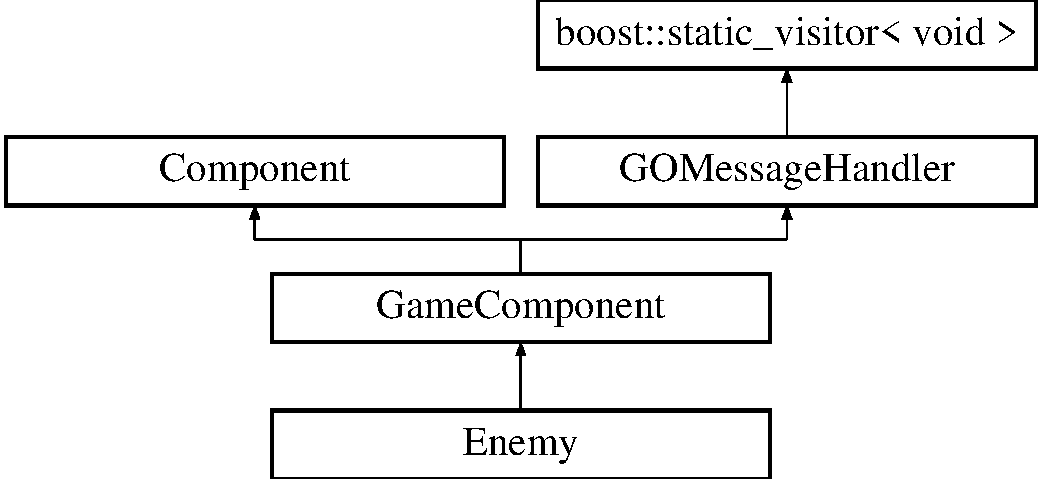
\includegraphics[height=4.000000cm]{class_enemy}
\end{center}
\end{figure}
\subsection*{Public Member Functions}
\begin{DoxyCompactItemize}
\item 
\hypertarget{class_enemy_ae7858f3f39ec6e48b741b7a8eaff6c1d}{}\label{class_enemy_ae7858f3f39ec6e48b741b7a8eaff6c1d} 
{\bfseries Enemy} (\hyperlink{class_game_object}{Game\+Object} $\ast$)
\item 
\hypertarget{class_enemy_a2966f61498d00e488697a80ef4447ebe}{}\label{class_enemy_a2966f61498d00e488697a80ef4447ebe} 
virtual void {\bfseries init} (int life=2, std\+::string=\char`\"{}Enemy1.\+txt\char`\"{}, float speed=1.\+0)
\item 
\hypertarget{class_enemy_ad55ee71b5a8c23fbd00b3c368b90cc64}{}\label{class_enemy_ad55ee71b5a8c23fbd00b3c368b90cc64} 
virtual void {\bfseries update} ()
\item 
\hypertarget{class_enemy_a932135eb4e5987c4e873b4e55a5bf215}{}\label{class_enemy_a932135eb4e5987c4e873b4e55a5bf215} 
virtual void {\bfseries operator()} (\hyperlink{struct_d_e_s_t_r_o_y}{D\+E\+S\+T\+R\+OY} const \&e)
\item 
\hypertarget{class_enemy_a187b85da2861026493d68c81fb4ce5b9}{}\label{class_enemy_a187b85da2861026493d68c81fb4ce5b9} 
virtual void {\bfseries operator()} (\hyperlink{struct_c_h_a_n_g_e___l_i_f_e}{C\+H\+A\+N\+G\+E\+\_\+\+L\+I\+FE} const \&e)
\end{DoxyCompactItemize}
\subsection*{Protected Member Functions}
\begin{DoxyCompactItemize}
\item 
\hypertarget{class_enemy_a304c3d98161d2ebca4ddd8ce1ae974af}{}\label{class_enemy_a304c3d98161d2ebca4ddd8ce1ae974af} 
void {\bfseries init\+Values} (float speed)
\item 
\hypertarget{class_enemy_ae8740856fd04d64259d0bad0eb7ae3ce}{}\label{class_enemy_ae8740856fd04d64259d0bad0eb7ae3ce} 
void {\bfseries init\+Components} (int life\+Value, std\+::string path)
\item 
\hypertarget{class_enemy_a9a398f8d12234f02563b27440aff7891}{}\label{class_enemy_a9a398f8d12234f02563b27440aff7891} 
void {\bfseries move} ()
\end{DoxyCompactItemize}
\subsection*{Protected Attributes}
\begin{DoxyCompactItemize}
\item 
\hypertarget{class_enemy_a5ad8a827b28dd24331a434d1993d5c01}{}\label{class_enemy_a5ad8a827b28dd24331a434d1993d5c01} 
float {\bfseries \+\_\+speed}
\end{DoxyCompactItemize}


The documentation for this class was generated from the following files\+:\begin{DoxyCompactItemize}
\item 
F\+:/\+\_\+\+\_\+\+M\+A\+R\+T\+I\+N/\+\_\+\+\_\+\+E\+N\+J\+M\+I\+N/\+Projets/ascii/shooter/\+A\+S\+C\+I\+I\+\_\+\+S\+H\+O\+O\+T\+E\+R\+\_\+\+P\+R\+O\+T\+O/Enemy.\+h\item 
F\+:/\+\_\+\+\_\+\+M\+A\+R\+T\+I\+N/\+\_\+\+\_\+\+E\+N\+J\+M\+I\+N/\+Projets/ascii/shooter/\+A\+S\+C\+I\+I\+\_\+\+S\+H\+O\+O\+T\+E\+R\+\_\+\+P\+R\+O\+T\+O/Enemy.\+cpp\end{DoxyCompactItemize}

\hypertarget{class_game}{}\section{Game Class Reference}
\label{class_game}\index{Game@{Game}}
Inheritance diagram for Game\+:\begin{figure}[H]
\begin{center}
\leavevmode
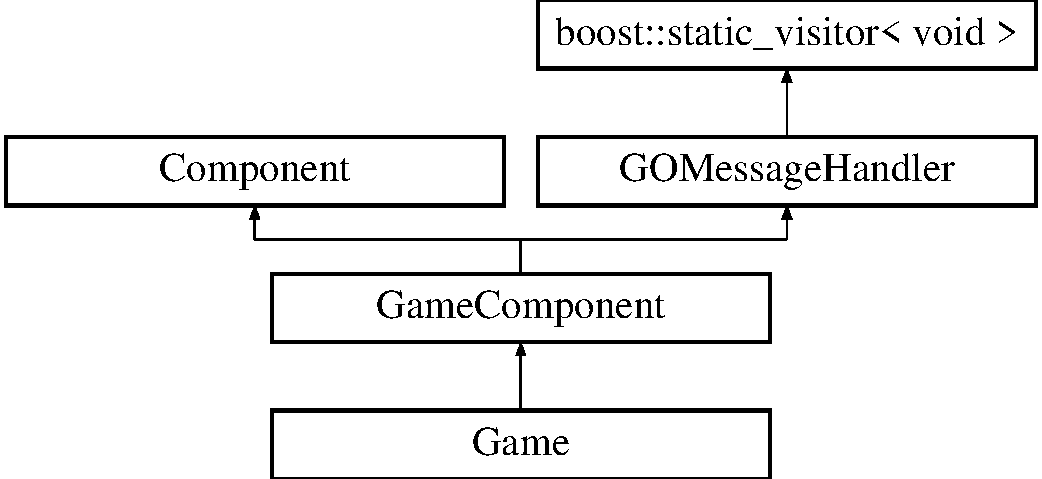
\includegraphics[height=4.000000cm]{class_game}
\end{center}
\end{figure}
\subsection*{Public Member Functions}
\begin{DoxyCompactItemize}
\item 
\hyperlink{class_game_a366e0d372a100b7de351caf14cede996}{Game} (\hyperlink{class_game_object}{Game\+Object} $\ast$)
\item 
\hypertarget{class_game_a6f3a33940524b6ba9d83f627ccb14bbf}{}\label{class_game_a6f3a33940524b6ba9d83f627ccb14bbf} 
virtual void \hyperlink{class_game_a6f3a33940524b6ba9d83f627ccb14bbf}{init} ()
\begin{DoxyCompactList}\small\item\em initialise le joueur et le generateur d\textquotesingle{}enemis \end{DoxyCompactList}\item 
\hypertarget{class_game_a79df6376b332d63c9eca0dcee30305c3}{}\label{class_game_a79df6376b332d63c9eca0dcee30305c3} 
virtual void \hyperlink{class_game_a79df6376b332d63c9eca0dcee30305c3}{update} ()
\begin{DoxyCompactList}\small\item\em gere les inputs pour mettre le jeu en pause Gere l\textquotesingle{}apparition des enemis \end{DoxyCompactList}\end{DoxyCompactItemize}
\subsection*{Protected Member Functions}
\begin{DoxyCompactItemize}
\item 
\hypertarget{class_game_a405c0bb8156590c93304f11cf1f08065}{}\label{class_game_a405c0bb8156590c93304f11cf1f08065} 
void {\bfseries init\+Player} ()
\item 
\hypertarget{class_game_ab6ac1ec04e03f55c0af1d4f9d0540cc7}{}\label{class_game_ab6ac1ec04e03f55c0af1d4f9d0540cc7} 
void {\bfseries handle\+Inputs} ()
\item 
\hypertarget{class_game_a8e042746fe9490afb380d6bddcfbe140}{}\label{class_game_a8e042746fe9490afb380d6bddcfbe140} 
void {\bfseries init\+Enemy\+Generator} ()
\item 
\hypertarget{class_game_a14753444a9131fdd5985443584b05b08}{}\label{class_game_a14753444a9131fdd5985443584b05b08} 
void {\bfseries handle\+Enemies} ()
\item 
\hypertarget{class_game_a2e05059d70edc32d1d37a9fc1c179b86}{}\label{class_game_a2e05059d70edc32d1d37a9fc1c179b86} 
void {\bfseries spawn\+Enemy} (\hyperlink{structvector2}{vector2} position)
\end{DoxyCompactItemize}
\subsection*{Protected Attributes}
\begin{DoxyCompactItemize}
\item 
\hypertarget{class_game_a24743764a183ce755b12282940d5aa9d}{}\label{class_game_a24743764a183ce755b12282940d5aa9d} 
double {\bfseries \+\_\+enemy\+Spawn\+Rate}
\item 
\hypertarget{class_game_a28155935797d67083587e848effc1eb8}{}\label{class_game_a28155935797d67083587e848effc1eb8} 
\hyperlink{class_n_y_timer}{N\+Y\+Timer} $\ast$ {\bfseries \+\_\+timer}
\item 
\hypertarget{class_game_a4bcab81144d9676362e8e964337e43a1}{}\label{class_game_a4bcab81144d9676362e8e964337e43a1} 
double {\bfseries \+\_\+previous}
\item 
\hypertarget{class_game_a546c6124b218181cac529da2bcf47de4}{}\label{class_game_a546c6124b218181cac529da2bcf47de4} 
double {\bfseries \+\_\+elapsed}
\item 
\hypertarget{class_game_a82b8447c7ca1d8a6114f97fb15bbcc00}{}\label{class_game_a82b8447c7ca1d8a6114f97fb15bbcc00} 
std\+::default\+\_\+random\+\_\+engine {\bfseries \+\_\+generator}
\item 
\hypertarget{class_game_a7731391cbc79c28c8fbecf3ee4bf5ca5}{}\label{class_game_a7731391cbc79c28c8fbecf3ee4bf5ca5} 
std\+::bernoulli\+\_\+distribution {\bfseries \+\_\+bernouilli\+Distribution}
\item 
\hypertarget{class_game_a20a7cd8706d26ec0c45bbe52f84b2e81}{}\label{class_game_a20a7cd8706d26ec0c45bbe52f84b2e81} 
std\+::uniform\+\_\+int\+\_\+distribution$<$ int $>$ {\bfseries \+\_\+uniform\+Distribution}
\end{DoxyCompactItemize}


\subsection{Constructor \& Destructor Documentation}
\hypertarget{class_game_a366e0d372a100b7de351caf14cede996}{}\label{class_game_a366e0d372a100b7de351caf14cede996} 
\index{Game@{Game}!Game@{Game}}
\index{Game@{Game}!Game@{Game}}
\subsubsection{\texorpdfstring{Game()}{Game()}}
{\footnotesize\ttfamily Game\+::\+Game (\begin{DoxyParamCaption}\item[{\hyperlink{class_game_object}{Game\+Object} $\ast$}]{obj }\end{DoxyParamCaption})}

cf. constructeur de \hyperlink{class_game_component}{Game\+Component} 

The documentation for this class was generated from the following files\+:\begin{DoxyCompactItemize}
\item 
F\+:/\+\_\+\+\_\+\+M\+A\+R\+T\+I\+N/\+\_\+\+\_\+\+E\+N\+J\+M\+I\+N/\+Projets/ascii/shooter/\+A\+S\+C\+I\+I\+\_\+\+S\+H\+O\+O\+T\+E\+R\+\_\+\+P\+R\+O\+T\+O/Game.\+h\item 
F\+:/\+\_\+\+\_\+\+M\+A\+R\+T\+I\+N/\+\_\+\+\_\+\+E\+N\+J\+M\+I\+N/\+Projets/ascii/shooter/\+A\+S\+C\+I\+I\+\_\+\+S\+H\+O\+O\+T\+E\+R\+\_\+\+P\+R\+O\+T\+O/Game.\+cpp\end{DoxyCompactItemize}

\hypertarget{class_game_component}{}\section{Game\+Component Class Reference}
\label{class_game_component}\index{Game\+Component@{Game\+Component}}


Classe de base des scripts utilisateurs.  




{\ttfamily \#include $<$Game\+Component.\+h$>$}

Inheritance diagram for Game\+Component\+:\begin{figure}[H]
\begin{center}
\leavevmode
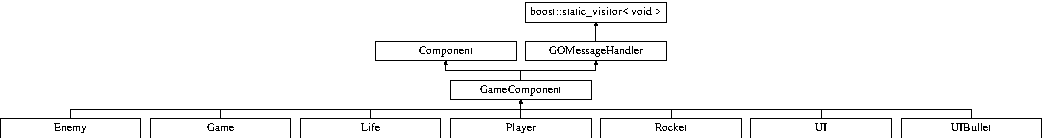
\includegraphics[height=1.839080cm]{class_game_component}
\end{center}
\end{figure}
\subsection*{Public Member Functions}
\begin{DoxyCompactItemize}
\item 
\hyperlink{class_game_component_a7d6d7a04c69a2eb0aa2d367925b501a2}{Game\+Component} (\hyperlink{class_game_object}{Game\+Object} $\ast$obj)
\begin{DoxyCompactList}\small\item\em Constructeur de \hyperlink{class_game_component}{Game\+Component} qui enregistre le \hyperlink{class_game_object}{Game\+Object} qui le contient. \end{DoxyCompactList}\item 
\hypertarget{class_game_component_ae602abc2eed3c565f410548aad7ee14e}{}\label{class_game_component_ae602abc2eed3c565f410548aad7ee14e} 
virtual void \hyperlink{class_game_component_ae602abc2eed3c565f410548aad7ee14e}{init} ()
\begin{DoxyCompactList}\small\item\em Initialise le \hyperlink{class_game_component}{Game\+Component}. \end{DoxyCompactList}\item 
\hypertarget{class_game_component_a3334ffc79f717357970abfbdb7eb4024}{}\label{class_game_component_a3334ffc79f717357970abfbdb7eb4024} 
virtual void \hyperlink{class_game_component_a3334ffc79f717357970abfbdb7eb4024}{wake} ()
\begin{DoxyCompactList}\small\item\em Reset le \hyperlink{class_game_component}{Game\+Component}. \end{DoxyCompactList}\item 
\hypertarget{class_game_component_a65fc004cd4dc7593052327ff874bb2f0}{}\label{class_game_component_a65fc004cd4dc7593052327ff874bb2f0} 
virtual void \hyperlink{class_game_component_a65fc004cd4dc7593052327ff874bb2f0}{update} ()=0
\begin{DoxyCompactList}\small\item\em Update le \hyperlink{class_game_component}{Game\+Component} a chaque tick. \end{DoxyCompactList}\item 
\hypertarget{class_game_component_a30bad20d9395895883bb75b998e9c974}{}\label{class_game_component_a30bad20d9395895883bb75b998e9c974} 
void \hyperlink{class_game_component_a30bad20d9395895883bb75b998e9c974}{send\+Message} (G\+O\+Message)
\begin{DoxyCompactList}\small\item\em Envoie un message au \hyperlink{class_game_object}{Game\+Object}. \end{DoxyCompactList}\item 
virtual void \hyperlink{class_game_component_a449c4a683e9bb42e0ab939a06e7b0640}{receive\+Message} (G\+O\+Message)
\begin{DoxyCompactList}\small\item\em Recoit et traite un message. \end{DoxyCompactList}\end{DoxyCompactItemize}
\subsection*{Protected Member Functions}
\begin{DoxyCompactItemize}
\item 
\hypertarget{class_game_component_abeecc14e2cd29b7ec83d74aabfe4403b}{}\label{class_game_component_abeecc14e2cd29b7ec83d74aabfe4403b} 
\hyperlink{class_component}{Component} $\ast$ {\bfseries add\+Component} (\hyperlink{class_component}{Component} $\ast$)
\end{DoxyCompactItemize}
\subsection*{Additional Inherited Members}


\subsection{Detailed Description}
Classe de base des scripts utilisateurs. 

Offre une interface pour les fonctionalites de base des scripts utilisateurs 

\subsection{Constructor \& Destructor Documentation}
\hypertarget{class_game_component_a7d6d7a04c69a2eb0aa2d367925b501a2}{}\label{class_game_component_a7d6d7a04c69a2eb0aa2d367925b501a2} 
\index{Game\+Component@{Game\+Component}!Game\+Component@{Game\+Component}}
\index{Game\+Component@{Game\+Component}!Game\+Component@{Game\+Component}}
\subsubsection{\texorpdfstring{Game\+Component()}{GameComponent()}}
{\footnotesize\ttfamily Game\+Component\+::\+Game\+Component (\begin{DoxyParamCaption}\item[{\hyperlink{class_game_object}{Game\+Object} $\ast$}]{obj }\end{DoxyParamCaption})}



Constructeur de \hyperlink{class_game_component}{Game\+Component} qui enregistre le \hyperlink{class_game_object}{Game\+Object} qui le contient. 


\begin{DoxyParams}{Parameters}
{\em Un} & pointeur vers un \hyperlink{class_game_object}{Game\+Object} \\
\hline
\end{DoxyParams}


\subsection{Member Function Documentation}
\hypertarget{class_game_component_a449c4a683e9bb42e0ab939a06e7b0640}{}\label{class_game_component_a449c4a683e9bb42e0ab939a06e7b0640} 
\index{Game\+Component@{Game\+Component}!receive\+Message@{receive\+Message}}
\index{receive\+Message@{receive\+Message}!Game\+Component@{Game\+Component}}
\subsubsection{\texorpdfstring{receive\+Message()}{receiveMessage()}}
{\footnotesize\ttfamily void Game\+Component\+::receive\+Message (\begin{DoxyParamCaption}\item[{G\+O\+Message}]{message }\end{DoxyParamCaption})\hspace{0.3cm}{\ttfamily [virtual]}}



Recoit et traite un message. 


\begin{DoxyParams}{Parameters}
{\em Un} & message a traiter \\
\hline
\end{DoxyParams}


The documentation for this class was generated from the following files\+:\begin{DoxyCompactItemize}
\item 
F\+:/\+\_\+\+\_\+\+M\+A\+R\+T\+I\+N/\+\_\+\+\_\+\+E\+N\+J\+M\+I\+N/\+Projets/ascii/shooter/\+A\+S\+C\+I\+I\+\_\+\+S\+H\+O\+O\+T\+E\+R\+\_\+\+P\+R\+O\+T\+O/Game\+Component.\+h\item 
F\+:/\+\_\+\+\_\+\+M\+A\+R\+T\+I\+N/\+\_\+\+\_\+\+E\+N\+J\+M\+I\+N/\+Projets/ascii/shooter/\+A\+S\+C\+I\+I\+\_\+\+S\+H\+O\+O\+T\+E\+R\+\_\+\+P\+R\+O\+T\+O/Game\+Component.\+cpp\end{DoxyCompactItemize}

\hypertarget{class_game_engine}{}\section{Game\+Engine Class Reference}
\label{class_game_engine}\index{Game\+Engine@{Game\+Engine}}


{\ttfamily \#include $<$Game\+Engine.\+h$>$}

\subsection*{Public Member Functions}
\begin{DoxyCompactItemize}
\item 
\hypertarget{class_game_engine_a5505704cb9ba58c5d029d8a736eff73d}{}\label{class_game_engine_a5505704cb9ba58c5d029d8a736eff73d} 
void {\bfseries add\+Scene} (\hyperlink{class_scene}{Scene} $\ast$scene)
\item 
\hypertarget{class_game_engine_aba1c35007c56a3082102f67c08ea5580}{}\label{class_game_engine_aba1c35007c56a3082102f67c08ea5580} 
void {\bfseries define\+Starting\+Scene} (std\+::string name)
\item 
\hypertarget{class_game_engine_ad2bb379da2ce51978a989de4ca979ecb}{}\label{class_game_engine_ad2bb379da2ce51978a989de4ca979ecb} 
void {\bfseries define\+Starting\+Scene} (\hyperlink{class_scene}{Scene} $\ast$scene)
\item 
\hypertarget{class_game_engine_a8116aae790eaf236907d5d75401cd628}{}\label{class_game_engine_a8116aae790eaf236907d5d75401cd628} 
\hyperlink{class_scene}{Scene} $\ast$ {\bfseries get\+Current\+Scene} ()
\item 
\hypertarget{class_game_engine_ac70d59f0de33c34f84863a550408a476}{}\label{class_game_engine_ac70d59f0de33c34f84863a550408a476} 
\hyperlink{class_scene}{Scene} $\ast$ {\bfseries get\+Scene} (std\+::string name)
\item 
\hypertarget{class_game_engine_a000c4cc070830d727f349b094ab402e3}{}\label{class_game_engine_a000c4cc070830d727f349b094ab402e3} 
void {\bfseries switch\+Scene} (std\+::string new\+Scene)
\item 
\hypertarget{class_game_engine_aef45d9ee461773587e266c57783de1a3}{}\label{class_game_engine_aef45d9ee461773587e266c57783de1a3} 
void {\bfseries send\+Message} (S\+C\+Message message)
\item 
\hypertarget{class_game_engine_ab01970da2c68fefbf48b98c59d5627ae}{}\label{class_game_engine_ab01970da2c68fefbf48b98c59d5627ae} 
void {\bfseries run} ()
\item 
\hypertarget{class_game_engine_a0ddc45d96adc0373346663302e429b12}{}\label{class_game_engine_a0ddc45d96adc0373346663302e429b12} 
std\+::vector$<$ \hyperlink{class_game_object}{Game\+Object} $\ast$ $>$ $\ast$ {\bfseries get\+Objects} ()
\item 
\hypertarget{class_game_engine_a5881933816240d7c21d66383ad3abdae}{}\label{class_game_engine_a5881933816240d7c21d66383ad3abdae} 
\hyperlink{class_game_object}{Game\+Object} $\ast$ {\bfseries get\+New\+Game\+Object} (std\+::string name, \hyperlink{structvector2}{vector2} position=\{ 0, 0 \})
\item 
\hypertarget{class_game_engine_a93ae1a7543981d2d3d0e70b14174135f}{}\label{class_game_engine_a93ae1a7543981d2d3d0e70b14174135f} 
void {\bfseries add\+New\+Objects} ()
\item 
\hypertarget{class_game_engine_a49e995c66c1c09394c75d31cbea4b691}{}\label{class_game_engine_a49e995c66c1c09394c75d31cbea4b691} 
void {\bfseries pass\+Object} (\hyperlink{class_game_object}{Game\+Object} $\ast$)
\item 
\hypertarget{class_game_engine_a92a0f7ffa3e36c93b51427dcf36a2586}{}\label{class_game_engine_a92a0f7ffa3e36c93b51427dcf36a2586} 
\hyperlink{class_game_object}{Game\+Object} $\ast$ {\bfseries find\+Object\+With\+Tag} (std\+::string tag)
\item 
\hypertarget{class_game_engine_ad82b626def2e52b28f0d6c2d167589f6}{}\label{class_game_engine_ad82b626def2e52b28f0d6c2d167589f6} 
void {\bfseries quit} ()
\end{DoxyCompactItemize}
\subsection*{Static Public Member Functions}
\begin{DoxyCompactItemize}
\item 
\hypertarget{class_game_engine_a5d5df5f1dabaaa1b98eeb1340f4f118d}{}\label{class_game_engine_a5d5df5f1dabaaa1b98eeb1340f4f118d} 
static \hyperlink{class_game_engine}{Game\+Engine} \& {\bfseries instance} ()
\end{DoxyCompactItemize}
\subsection*{Public Attributes}
\begin{DoxyCompactItemize}
\item 
\hypertarget{class_game_engine_a8d1a51bb0bd082dfddfbcc25bae08ace}{}\label{class_game_engine_a8d1a51bb0bd082dfddfbcc25bae08ace} 
\hyperlink{class_input_engine}{Input\+Engine} $\ast$ {\bfseries \+\_\+inputs}
\item 
\hypertarget{class_game_engine_a84532de3912402092e41bded12137b44}{}\label{class_game_engine_a84532de3912402092e41bded12137b44} 
\hyperlink{class_n_y_timer}{N\+Y\+Timer} {\bfseries \+\_\+timer}
\end{DoxyCompactItemize}
\subsection*{Protected Member Functions}
\begin{DoxyCompactItemize}
\item 
\hypertarget{class_game_engine_a3577e939b14e8cb0677d508f2f6a6912}{}\label{class_game_engine_a3577e939b14e8cb0677d508f2f6a6912} 
{\bfseries Game\+Engine} (\hyperlink{class_game_engine}{Game\+Engine} const \&)=delete
\item 
\hypertarget{class_game_engine_af1220370747be0fc7c4ca78c089c08c3}{}\label{class_game_engine_af1220370747be0fc7c4ca78c089c08c3} 
void {\bfseries operator=} (\hyperlink{class_game_engine}{Game\+Engine} const \&)=delete
\item 
\hypertarget{class_game_engine_af45dfb1c31ce79d53b00eace85c68063}{}\label{class_game_engine_af45dfb1c31ce79d53b00eace85c68063} 
void {\bfseries reset\+Time} ()
\item 
\hypertarget{class_game_engine_a2a1ee54e0b6fc398feab0597fabf2713}{}\label{class_game_engine_a2a1ee54e0b6fc398feab0597fabf2713} 
void {\bfseries go\+To\+Next\+Scene} ()
\item 
\hypertarget{class_game_engine_a3caea6165710b1cf54c392ee803891c7}{}\label{class_game_engine_a3caea6165710b1cf54c392ee803891c7} 
void {\bfseries go\+To\+Previous\+Scene} ()
\item 
\hypertarget{class_game_engine_a9cf603b0eaae873e5513f752aa2b6fe5}{}\label{class_game_engine_a9cf603b0eaae873e5513f752aa2b6fe5} 
void {\bfseries clean\+Current\+Scene} ()
\item 
\hypertarget{class_game_engine_ae03241b464040b659b6a91f27920e8c3}{}\label{class_game_engine_ae03241b464040b659b6a91f27920e8c3} 
void {\bfseries update} ()
\item 
\hypertarget{class_game_engine_aa79933550f7680ffe62035f5c3181b55}{}\label{class_game_engine_aa79933550f7680ffe62035f5c3181b55} 
void {\bfseries update\+Physics} ()
\item 
\hypertarget{class_game_engine_a267bf9164ba09e32b7a24ba4afb527d4}{}\label{class_game_engine_a267bf9164ba09e32b7a24ba4afb527d4} 
void {\bfseries render} ()
\end{DoxyCompactItemize}
\subsection*{Protected Attributes}
\begin{DoxyCompactItemize}
\item 
\hypertarget{class_game_engine_a6bb48df06765a1d31310e0bbcf582b2b}{}\label{class_game_engine_a6bb48df06765a1d31310e0bbcf582b2b} 
bool {\bfseries \+\_\+switch\+Scene}
\item 
\hypertarget{class_game_engine_a0ebfd3cc173547a668e763b72449dcc3}{}\label{class_game_engine_a0ebfd3cc173547a668e763b72449dcc3} 
std\+::vector$<$ \hyperlink{class_game_object}{Game\+Object} $\ast$ $>$ {\bfseries \+\_\+new\+Objects}
\item 
\hypertarget{class_game_engine_a857a6cf409bd4697a0ee31238e74b670}{}\label{class_game_engine_a857a6cf409bd4697a0ee31238e74b670} 
vector$<$ \hyperlink{class_scene}{Scene} $\ast$ $>$ {\bfseries \+\_\+scenes}
\item 
\hypertarget{class_game_engine_a0ed9d4b010faefc0fc16b6381c0fd77c}{}\label{class_game_engine_a0ed9d4b010faefc0fc16b6381c0fd77c} 
\hyperlink{class_scene}{Scene} $\ast$ {\bfseries \+\_\+previous\+Scene}
\item 
\hypertarget{class_game_engine_a8d2b7530557db9bcff501fe39cc65539}{}\label{class_game_engine_a8d2b7530557db9bcff501fe39cc65539} 
\hyperlink{class_scene}{Scene} $\ast$ {\bfseries \+\_\+current\+Scene}
\item 
\hypertarget{class_game_engine_a774d8b94d3f52f0387de3eba6804dfa9}{}\label{class_game_engine_a774d8b94d3f52f0387de3eba6804dfa9} 
\hyperlink{class_scene}{Scene} $\ast$ {\bfseries \+\_\+next\+Scene}
\item 
\hypertarget{class_game_engine_aa5a6689bfdebff663b691dfbf64596ec}{}\label{class_game_engine_aa5a6689bfdebff663b691dfbf64596ec} 
std\+::vector$<$ \hyperlink{class_game_object}{Game\+Object} $\ast$ $>$ {\bfseries \+\_\+passing\+Game\+Objects}
\item 
\hypertarget{class_game_engine_a356588004d68586f945ae85bc5060700}{}\label{class_game_engine_a356588004d68586f945ae85bc5060700} 
\hyperlink{class_graphics_engine}{Graphics\+Engine} $\ast$ {\bfseries \+\_\+graphics}
\item 
\hypertarget{class_game_engine_a913f0eb92dda8fc1cd4cec59b9f7c580}{}\label{class_game_engine_a913f0eb92dda8fc1cd4cec59b9f7c580} 
\hyperlink{class_physics_engine}{Physics\+Engine} $\ast$ {\bfseries \+\_\+physics}
\item 
\hypertarget{class_game_engine_a71cb9124b614680cdc4fbe6823900445}{}\label{class_game_engine_a71cb9124b614680cdc4fbe6823900445} 
double {\bfseries \+\_\+previous}
\item 
\hypertarget{class_game_engine_abe7083245b75ccd6969b54cde562167b}{}\label{class_game_engine_abe7083245b75ccd6969b54cde562167b} 
double {\bfseries \+\_\+lag}
\item 
\hypertarget{class_game_engine_a27abc89c39a79dd719084c2a9267d61d}{}\label{class_game_engine_a27abc89c39a79dd719084c2a9267d61d} 
double {\bfseries \+\_\+current}
\item 
\hypertarget{class_game_engine_a0a2ef0a08be4b7ac9f02e7db06f0bb50}{}\label{class_game_engine_a0a2ef0a08be4b7ac9f02e7db06f0bb50} 
double {\bfseries \+\_\+elapsed}
\item 
\hypertarget{class_game_engine_a6f8d9c72d09c8894b8ccbad014376285}{}\label{class_game_engine_a6f8d9c72d09c8894b8ccbad014376285} 
bool {\bfseries \+\_\+quit} = false
\end{DoxyCompactItemize}


\subsection{Detailed Description}
\hyperlink{class_game_engine}{Game\+Engine} Takes care of initiating the other engines and running the game Takes care of switching between scenes 

The documentation for this class was generated from the following files\+:\begin{DoxyCompactItemize}
\item 
F\+:/\+\_\+\+\_\+\+M\+A\+R\+T\+I\+N/\+\_\+\+\_\+\+E\+N\+J\+M\+I\+N/\+Projets/ascii/shooter/\+A\+S\+C\+I\+I\+\_\+\+S\+H\+O\+O\+T\+E\+R\+\_\+\+P\+R\+O\+T\+O/Game\+Engine.\+h\item 
F\+:/\+\_\+\+\_\+\+M\+A\+R\+T\+I\+N/\+\_\+\+\_\+\+E\+N\+J\+M\+I\+N/\+Projets/ascii/shooter/\+A\+S\+C\+I\+I\+\_\+\+S\+H\+O\+O\+T\+E\+R\+\_\+\+P\+R\+O\+T\+O/Game\+Engine.\+cpp\end{DoxyCompactItemize}

\hypertarget{class_game_object}{}\section{Game\+Object Class Reference}
\label{class_game_object}\index{Game\+Object@{Game\+Object}}


{\ttfamily \#include $<$Game\+Object.\+h$>$}

\subsection*{Public Member Functions}
\begin{DoxyCompactItemize}
\item 
\hypertarget{class_game_object_adbdcffa0cd72ae987c033e61f6b12880}{}\label{class_game_object_adbdcffa0cd72ae987c033e61f6b12880} 
{\bfseries Game\+Object} (std\+::string tag, \hyperlink{structvector2}{vector2} position=\{ 0, 0 \})
\item 
void \hyperlink{class_game_object_adad7d284b670db722a2fda8e6a7997e3}{update} ()
\begin{DoxyCompactList}\small\item\em Update le \hyperlink{class_game_object}{Game\+Object}. \end{DoxyCompactList}\item 
void \hyperlink{class_game_object_a0d68cf2723dd5cedc12579c08c97df04}{add\+Component} (\hyperlink{class_component}{Component} $\ast$)
\begin{DoxyCompactList}\small\item\em Ajoute un \hyperlink{class_component}{Component} au \hyperlink{class_game_object}{Game\+Object}. \end{DoxyCompactList}\item 
std\+::vector$<$ \hyperlink{class_component}{Component} $\ast$ $>$ \& \hyperlink{class_game_object_addbe774c69d6fb3b50acbef5f74d7319}{get\+Components} ()
\begin{DoxyCompactList}\small\item\em Recupere la liste des \hyperlink{class_component}{Component}. \end{DoxyCompactList}\item 
{\footnotesize template$<$class T $>$ }\\T $\ast$ \hyperlink{class_game_object_a1c50376c7f24439359a3962f57dfd513}{get\+Component} ()
\begin{DoxyCompactList}\small\item\em Recupere un \hyperlink{class_component}{Component}  Le type de \hyperlink{class_component}{Component} que l\textquotesingle{}on veut recuperer. \end{DoxyCompactList}\item 
std\+::string \hyperlink{class_game_object_a7a7cc496716e8c8453bd0bb954f2a7ee}{get\+Name} ()
\begin{DoxyCompactList}\small\item\em Donne le nom du \hyperlink{class_game_object}{Game\+Object}. \end{DoxyCompactList}\item 
void \hyperlink{class_game_object_a58a24ffbffbcd03afa926b2c01d545fe}{set\+Name} (std\+::string name)
\begin{DoxyCompactList}\small\item\em Set le nom du \hyperlink{class_game_object}{Game\+Object}. \end{DoxyCompactList}\item 
void \hyperlink{class_game_object_abdc20833ca1a65acd819888247216929}{send\+Message} (const G\+O\+Message) const
\begin{DoxyCompactList}\small\item\em Envoie d\textquotesingle{}un message. \end{DoxyCompactList}\item 
bool \hyperlink{class_game_object_aaac5b633ac19e0facea0b7cb6f93ccef}{is\+Tagged} (std\+::string tag)
\begin{DoxyCompactList}\small\item\em Test sur le tag de l\textquotesingle{}object. \end{DoxyCompactList}\item 
std\+::string \hyperlink{class_game_object_a099a32d11225032f9a1a35d15a307a27}{get\+Tag} ()
\item 
void \hyperlink{class_game_object_a2c5d76ea1ebd18e6c3e74cdd680ed349}{set\+Tag} (std\+::string tag)
\begin{DoxyCompactList}\small\item\em Set le tag du \hyperlink{class_game_object}{Game\+Object}. \end{DoxyCompactList}\item 
void \hyperlink{class_game_object_af54107b086de78b1fc6190088bdfb468}{kill} ()
\begin{DoxyCompactList}\small\item\em Marque le \hyperlink{class_game_object}{Game\+Object} comme mort, il sera supprime par le \hyperlink{class_game_engine}{Game\+Engine} lors de la tick suivante. \end{DoxyCompactList}\item 
bool \hyperlink{class_game_object_af509340fc9f95d8d39afe7ec63d90128}{is\+Dead} ()
\begin{DoxyCompactList}\small\item\em Donne l\textquotesingle{}etat de vie du \hyperlink{class_game_object}{Game\+Object}. \end{DoxyCompactList}\end{DoxyCompactItemize}
\subsection*{Static Public Member Functions}
\begin{DoxyCompactItemize}
\item 
static bool \hyperlink{class_game_object_a2ceae5dbcdd0e8621d08c6c461068a2b}{find\+Tag} (std\+::string tag)
\begin{DoxyCompactList}\small\item\em Methode de classe qui recherche si le tag existe (si un object a deja utilise le tag) \end{DoxyCompactList}\end{DoxyCompactItemize}
\subsection*{Public Attributes}
\begin{DoxyCompactItemize}
\item 
\hypertarget{class_game_object_a86822412aab633fe5a2a78678fdf55b7}{}\label{class_game_object_a86822412aab633fe5a2a78678fdf55b7} 
\hyperlink{structvector2}{vector2} \hyperlink{class_game_object_a86822412aab633fe5a2a78678fdf55b7}{\+\_\+position}
\begin{DoxyCompactList}\small\item\em Position de l\textquotesingle{}objet. \end{DoxyCompactList}\item 
\hypertarget{class_game_object_ac1f91cb46f40c3b254505d66a9da1653}{}\label{class_game_object_ac1f91cb46f40c3b254505d66a9da1653} 
bool \hyperlink{class_game_object_ac1f91cb46f40c3b254505d66a9da1653}{\+\_\+enabled}
\begin{DoxyCompactList}\small\item\em etat d\textquotesingle{}activation de l\textquotesingle{}objet \end{DoxyCompactList}\end{DoxyCompactItemize}


\subsection{Detailed Description}
Recuperation a partir du \hyperlink{class_game_engine}{Game\+Engine}, qui ajoute directement l\textquotesingle{}object a la scene courante Conteneur de componsants, Ajout de composants au \hyperlink{class_game_object}{Game\+Object}, qui representent \+:
\begin{DoxyItemize}
\item Soit des fonctions de base (physique, graphique)
\item Soit des scripts permet d\textquotesingle{}obtenir des comportements pour complexes 
\end{DoxyItemize}

\subsection{Member Function Documentation}
\hypertarget{class_game_object_a0d68cf2723dd5cedc12579c08c97df04}{}\label{class_game_object_a0d68cf2723dd5cedc12579c08c97df04} 
\index{Game\+Object@{Game\+Object}!add\+Component@{add\+Component}}
\index{add\+Component@{add\+Component}!Game\+Object@{Game\+Object}}
\subsubsection{\texorpdfstring{add\+Component()}{addComponent()}}
{\footnotesize\ttfamily void Game\+Object\+::add\+Component (\begin{DoxyParamCaption}\item[{\hyperlink{class_component}{Component} $\ast$}]{c }\end{DoxyParamCaption})}



Ajoute un \hyperlink{class_component}{Component} au \hyperlink{class_game_object}{Game\+Object}. 

Le \hyperlink{class_component}{Component} passe en parametre est ajoute a la liste de componsants du \hyperlink{class_game_object}{Game\+Object}


\begin{DoxyParams}{Parameters}
{\em Pointeur} & sur \hyperlink{class_component}{Component} \\
\hline
\end{DoxyParams}
\hypertarget{class_game_object_a2ceae5dbcdd0e8621d08c6c461068a2b}{}\label{class_game_object_a2ceae5dbcdd0e8621d08c6c461068a2b} 
\index{Game\+Object@{Game\+Object}!find\+Tag@{find\+Tag}}
\index{find\+Tag@{find\+Tag}!Game\+Object@{Game\+Object}}
\subsubsection{\texorpdfstring{find\+Tag()}{findTag()}}
{\footnotesize\ttfamily bool Game\+Object\+::find\+Tag (\begin{DoxyParamCaption}\item[{std\+::string}]{tag }\end{DoxyParamCaption})\hspace{0.3cm}{\ttfamily [static]}}



Methode de classe qui recherche si le tag existe (si un object a deja utilise le tag) 


\begin{DoxyParams}{Parameters}
{\em le} & tag a rechercher \\
\hline
\end{DoxyParams}
\hypertarget{class_game_object_a1c50376c7f24439359a3962f57dfd513}{}\label{class_game_object_a1c50376c7f24439359a3962f57dfd513} 
\index{Game\+Object@{Game\+Object}!get\+Component@{get\+Component}}
\index{get\+Component@{get\+Component}!Game\+Object@{Game\+Object}}
\subsubsection{\texorpdfstring{get\+Component()}{getComponent()}}
{\footnotesize\ttfamily template$<$class T $>$ \\
T$\ast$ Game\+Object\+::get\+Component (\begin{DoxyParamCaption}{ }\end{DoxyParamCaption})\hspace{0.3cm}{\ttfamily [inline]}}



Recupere un \hyperlink{class_component}{Component}  Le type de \hyperlink{class_component}{Component} que l\textquotesingle{}on veut recuperer. 

\begin{DoxyReturn}{Returns}
Le premier \hyperlink{class_component}{Component} qui a pour type le Type T passe en parametre 
\end{DoxyReturn}
\hypertarget{class_game_object_addbe774c69d6fb3b50acbef5f74d7319}{}\label{class_game_object_addbe774c69d6fb3b50acbef5f74d7319} 
\index{Game\+Object@{Game\+Object}!get\+Components@{get\+Components}}
\index{get\+Components@{get\+Components}!Game\+Object@{Game\+Object}}
\subsubsection{\texorpdfstring{get\+Components()}{getComponents()}}
{\footnotesize\ttfamily vector$<$ \hyperlink{class_component}{Component} $\ast$ $>$ \& Game\+Object\+::get\+Components (\begin{DoxyParamCaption}{ }\end{DoxyParamCaption})}



Recupere la liste des \hyperlink{class_component}{Component}. 

\begin{DoxyReturn}{Returns}
Une r�f�rence vers le vector contenant les \hyperlink{class_component}{Component} du Game\+Objet 
\end{DoxyReturn}
\hypertarget{class_game_object_a7a7cc496716e8c8453bd0bb954f2a7ee}{}\label{class_game_object_a7a7cc496716e8c8453bd0bb954f2a7ee} 
\index{Game\+Object@{Game\+Object}!get\+Name@{get\+Name}}
\index{get\+Name@{get\+Name}!Game\+Object@{Game\+Object}}
\subsubsection{\texorpdfstring{get\+Name()}{getName()}}
{\footnotesize\ttfamily std\+::string Game\+Object\+::get\+Name (\begin{DoxyParamCaption}{ }\end{DoxyParamCaption})\hspace{0.3cm}{\ttfamily [inline]}}



Donne le nom du \hyperlink{class_game_object}{Game\+Object}. 

Le nom du \hyperlink{class_game_object}{Game\+Object} n\textquotesingle{}ai pas utilise par l\textquotesingle{}enjmin, il ne sert qu\textquotesingle{}a organiser le code si le client le desire

\begin{DoxyReturn}{Returns}
Le nom du \hyperlink{class_game_object}{Game\+Object} 
\end{DoxyReturn}
\hypertarget{class_game_object_a099a32d11225032f9a1a35d15a307a27}{}\label{class_game_object_a099a32d11225032f9a1a35d15a307a27} 
\index{Game\+Object@{Game\+Object}!get\+Tag@{get\+Tag}}
\index{get\+Tag@{get\+Tag}!Game\+Object@{Game\+Object}}
\subsubsection{\texorpdfstring{get\+Tag()}{getTag()}}
{\footnotesize\ttfamily string Game\+Object\+::get\+Tag (\begin{DoxyParamCaption}{ }\end{DoxyParamCaption})}

\begin{DoxyReturn}{Returns}
Le tag du \hyperlink{class_game_object}{Game\+Object} 
\end{DoxyReturn}
\hypertarget{class_game_object_af509340fc9f95d8d39afe7ec63d90128}{}\label{class_game_object_af509340fc9f95d8d39afe7ec63d90128} 
\index{Game\+Object@{Game\+Object}!is\+Dead@{is\+Dead}}
\index{is\+Dead@{is\+Dead}!Game\+Object@{Game\+Object}}
\subsubsection{\texorpdfstring{is\+Dead()}{isDead()}}
{\footnotesize\ttfamily bool Game\+Object\+::is\+Dead (\begin{DoxyParamCaption}{ }\end{DoxyParamCaption})\hspace{0.3cm}{\ttfamily [inline]}}



Donne l\textquotesingle{}etat de vie du \hyperlink{class_game_object}{Game\+Object}. 

Si la valeur de retour est false, le \hyperlink{class_game_object}{Game\+Object} sera supprime au tick suivant

\begin{DoxyReturn}{Returns}
true si le \hyperlink{class_game_object}{Game\+Object} est vivant, false sinon. 
\end{DoxyReturn}
\hypertarget{class_game_object_aaac5b633ac19e0facea0b7cb6f93ccef}{}\label{class_game_object_aaac5b633ac19e0facea0b7cb6f93ccef} 
\index{Game\+Object@{Game\+Object}!is\+Tagged@{is\+Tagged}}
\index{is\+Tagged@{is\+Tagged}!Game\+Object@{Game\+Object}}
\subsubsection{\texorpdfstring{is\+Tagged()}{isTagged()}}
{\footnotesize\ttfamily bool Game\+Object\+::is\+Tagged (\begin{DoxyParamCaption}\item[{std\+::string}]{tag }\end{DoxyParamCaption})}



Test sur le tag de l\textquotesingle{}object. 

Compare le tag de l\textquotesingle{}objet avec celui passe en parametre


\begin{DoxyParams}{Parameters}
{\em le} & tag a comparer \\
\hline
\end{DoxyParams}
\begin{DoxyReturn}{Returns}
true si les tags sont identiques, faux sinon 
\end{DoxyReturn}
\hypertarget{class_game_object_af54107b086de78b1fc6190088bdfb468}{}\label{class_game_object_af54107b086de78b1fc6190088bdfb468} 
\index{Game\+Object@{Game\+Object}!kill@{kill}}
\index{kill@{kill}!Game\+Object@{Game\+Object}}
\subsubsection{\texorpdfstring{kill()}{kill()}}
{\footnotesize\ttfamily void Game\+Object\+::kill (\begin{DoxyParamCaption}{ }\end{DoxyParamCaption})\hspace{0.3cm}{\ttfamily [inline]}}



Marque le \hyperlink{class_game_object}{Game\+Object} comme mort, il sera supprime par le \hyperlink{class_game_engine}{Game\+Engine} lors de la tick suivante. 

\hypertarget{class_game_object_abdc20833ca1a65acd819888247216929}{}\label{class_game_object_abdc20833ca1a65acd819888247216929} 
\index{Game\+Object@{Game\+Object}!send\+Message@{send\+Message}}
\index{send\+Message@{send\+Message}!Game\+Object@{Game\+Object}}
\subsubsection{\texorpdfstring{send\+Message()}{sendMessage()}}
{\footnotesize\ttfamily void Game\+Object\+::send\+Message (\begin{DoxyParamCaption}\item[{const G\+O\+Message}]{message }\end{DoxyParamCaption}) const}



Envoie d\textquotesingle{}un message. 

Fait passer le message a tous les \hyperlink{class_component}{Component} contenus dans le \hyperlink{class_game_object}{Game\+Object}


\begin{DoxyParams}{Parameters}
{\em Le} & message a envoyer \\
\hline
\end{DoxyParams}
\hypertarget{class_game_object_a58a24ffbffbcd03afa926b2c01d545fe}{}\label{class_game_object_a58a24ffbffbcd03afa926b2c01d545fe} 
\index{Game\+Object@{Game\+Object}!set\+Name@{set\+Name}}
\index{set\+Name@{set\+Name}!Game\+Object@{Game\+Object}}
\subsubsection{\texorpdfstring{set\+Name()}{setName()}}
{\footnotesize\ttfamily void Game\+Object\+::set\+Name (\begin{DoxyParamCaption}\item[{std\+::string}]{name }\end{DoxyParamCaption})\hspace{0.3cm}{\ttfamily [inline]}}



Set le nom du \hyperlink{class_game_object}{Game\+Object}. 

Le nom du \hyperlink{class_game_object}{Game\+Object} n\textquotesingle{}ai pas utilise par l\textquotesingle{}enjmin, il ne sert qu\textquotesingle{}a organiser le code si le client le desire


\begin{DoxyParams}{Parameters}
{\em Le} & nom du \hyperlink{class_game_object}{Game\+Object} \\
\hline
\end{DoxyParams}
\hypertarget{class_game_object_a2c5d76ea1ebd18e6c3e74cdd680ed349}{}\label{class_game_object_a2c5d76ea1ebd18e6c3e74cdd680ed349} 
\index{Game\+Object@{Game\+Object}!set\+Tag@{set\+Tag}}
\index{set\+Tag@{set\+Tag}!Game\+Object@{Game\+Object}}
\subsubsection{\texorpdfstring{set\+Tag()}{setTag()}}
{\footnotesize\ttfamily void Game\+Object\+::set\+Tag (\begin{DoxyParamCaption}\item[{std\+::string}]{tag }\end{DoxyParamCaption})}



Set le tag du \hyperlink{class_game_object}{Game\+Object}. 


\begin{DoxyParams}{Parameters}
{\em le} & nouveau nom du tag \\
\hline
\end{DoxyParams}
\hypertarget{class_game_object_adad7d284b670db722a2fda8e6a7997e3}{}\label{class_game_object_adad7d284b670db722a2fda8e6a7997e3} 
\index{Game\+Object@{Game\+Object}!update@{update}}
\index{update@{update}!Game\+Object@{Game\+Object}}
\subsubsection{\texorpdfstring{update()}{update()}}
{\footnotesize\ttfamily void Game\+Object\+::update (\begin{DoxyParamCaption}{ }\end{DoxyParamCaption})}



Update le \hyperlink{class_game_object}{Game\+Object}. 

Methode d\textquotesingle{}update, appelee a chaque tick par l\textquotesingle{}engine et qui appelle a son tour les update de tous les composants contenus dans le Game\+Obect 

The documentation for this class was generated from the following files\+:\begin{DoxyCompactItemize}
\item 
F\+:/\+\_\+\+\_\+\+M\+A\+R\+T\+I\+N/\+\_\+\+\_\+\+E\+N\+J\+M\+I\+N/\+Projets/ascii/shooter/\+A\+S\+C\+I\+I\+\_\+\+S\+H\+O\+O\+T\+E\+R\+\_\+\+P\+R\+O\+T\+O/Game\+Object.\+h\item 
F\+:/\+\_\+\+\_\+\+M\+A\+R\+T\+I\+N/\+\_\+\+\_\+\+E\+N\+J\+M\+I\+N/\+Projets/ascii/shooter/\+A\+S\+C\+I\+I\+\_\+\+S\+H\+O\+O\+T\+E\+R\+\_\+\+P\+R\+O\+T\+O/Game\+Object.\+cpp\end{DoxyCompactItemize}

\hypertarget{class_g_o_message_handler}{}\section{G\+O\+Message\+Handler Class Reference}
\label{class_g_o_message_handler}\index{G\+O\+Message\+Handler@{G\+O\+Message\+Handler}}
Inheritance diagram for G\+O\+Message\+Handler\+:\begin{figure}[H]
\begin{center}
\leavevmode
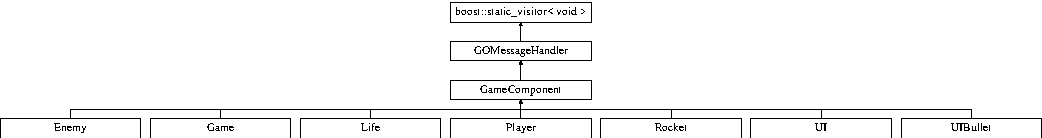
\includegraphics[height=1.839080cm]{class_g_o_message_handler}
\end{center}
\end{figure}
\subsection*{Public Member Functions}
\begin{DoxyCompactItemize}
\item 
\hypertarget{class_g_o_message_handler_a56185d82155d3917c046327978872668}{}\label{class_g_o_message_handler_a56185d82155d3917c046327978872668} 
virtual void {\bfseries operator()} (\hyperlink{struct_d_e_s_t_r_o_y}{D\+E\+S\+T\+R\+OY} const \&e)
\item 
\hypertarget{class_g_o_message_handler_a2fd424c1de0a2a7ed1b8d14f36a3fd57}{}\label{class_g_o_message_handler_a2fd424c1de0a2a7ed1b8d14f36a3fd57} 
virtual void {\bfseries operator()} (\hyperlink{struct_c_h_a_n_g_e___l_i_f_e}{C\+H\+A\+N\+G\+E\+\_\+\+L\+I\+FE} const \&e)
\item 
\hypertarget{class_g_o_message_handler_abb5fd98aec67539124ba38a95f0f3ef1}{}\label{class_g_o_message_handler_abb5fd98aec67539124ba38a95f0f3ef1} 
virtual void {\bfseries operator()} (\hyperlink{struct_u_i_c_o_n_t_e_x_t}{U\+I\+C\+O\+N\+T\+E\+XT} const \&e)
\end{DoxyCompactItemize}


The documentation for this class was generated from the following files\+:\begin{DoxyCompactItemize}
\item 
F\+:/\+\_\+\+\_\+\+M\+A\+R\+T\+I\+N/\+\_\+\+\_\+\+E\+N\+J\+M\+I\+N/\+Projets/ascii/shooter/\+A\+S\+C\+I\+I\+\_\+\+S\+H\+O\+O\+T\+E\+R\+\_\+\+P\+R\+O\+T\+O/Message\+Handler.\+h\item 
F\+:/\+\_\+\+\_\+\+M\+A\+R\+T\+I\+N/\+\_\+\+\_\+\+E\+N\+J\+M\+I\+N/\+Projets/ascii/shooter/\+A\+S\+C\+I\+I\+\_\+\+S\+H\+O\+O\+T\+E\+R\+\_\+\+P\+R\+O\+T\+O/Message\+Handler.\+cpp\end{DoxyCompactItemize}

\hypertarget{class_graphics_component}{}\section{Graphics\+Component Class Reference}
\label{class_graphics_component}\index{Graphics\+Component@{Graphics\+Component}}


\hyperlink{class_component}{Component} contenant un sprite a afficher dans la console.  




{\ttfamily \#include $<$Graphics\+Component.\+h$>$}

Inheritance diagram for Graphics\+Component\+:\begin{figure}[H]
\begin{center}
\leavevmode
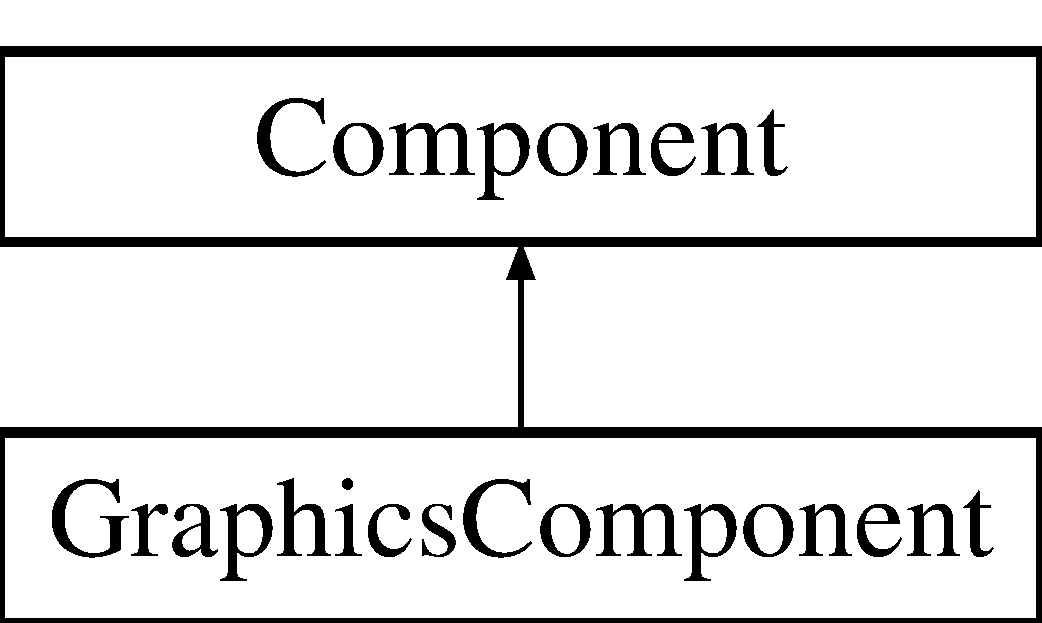
\includegraphics[height=2.000000cm]{class_graphics_component}
\end{center}
\end{figure}
\subsection*{Public Member Functions}
\begin{DoxyCompactItemize}
\item 
\hypertarget{class_graphics_component_a67fc1b715989a5e18d32e26b27a55c50}{}\label{class_graphics_component_a67fc1b715989a5e18d32e26b27a55c50} 
\hyperlink{class_graphics_component_a67fc1b715989a5e18d32e26b27a55c50}{Graphics\+Component} ()
\begin{DoxyCompactList}\small\item\em Creer un \hyperlink{class_graphics_component}{Graphics\+Component} par defaut, vide. \end{DoxyCompactList}\item 
\hyperlink{class_graphics_component_af9c775bcb7f51c76c25d32b3152cd5b2}{Graphics\+Component} (std\+::string path)
\begin{DoxyCompactList}\small\item\em Creer un \hyperlink{class_graphics_component}{Graphics\+Component} a partir d\textquotesingle{}un path vers un fichier texte. \end{DoxyCompactList}\item 
void \hyperlink{class_graphics_component_ab3e309ee0a8dcbc1b927d38bf2e1d8c9}{set\+Sprite} (std\+::string path)
\begin{DoxyCompactList}\small\item\em Set le sprite du \hyperlink{class_graphics_component}{Graphics\+Component} a partir d\textquotesingle{}un path vers un fichier texte. \end{DoxyCompactList}\end{DoxyCompactItemize}
\subsection*{Public Attributes}
\begin{DoxyCompactItemize}
\item 
\hypertarget{class_graphics_component_ab16775099a92f1442b2b2a1f41da997e}{}\label{class_graphics_component_ab16775099a92f1442b2b2a1f41da997e} 
std\+::vector$<$ \hyperlink{structpixel}{pixel} $>$ {\bfseries \+\_\+sprite}
\end{DoxyCompactItemize}


\subsection{Detailed Description}
\hyperlink{class_component}{Component} contenant un sprite a afficher dans la console. 

\subsection{Constructor \& Destructor Documentation}
\hypertarget{class_graphics_component_af9c775bcb7f51c76c25d32b3152cd5b2}{}\label{class_graphics_component_af9c775bcb7f51c76c25d32b3152cd5b2} 
\index{Graphics\+Component@{Graphics\+Component}!Graphics\+Component@{Graphics\+Component}}
\index{Graphics\+Component@{Graphics\+Component}!Graphics\+Component@{Graphics\+Component}}
\subsubsection{\texorpdfstring{Graphics\+Component()}{GraphicsComponent()}}
{\footnotesize\ttfamily Graphics\+Component\+::\+Graphics\+Component (\begin{DoxyParamCaption}\item[{std\+::string}]{path }\end{DoxyParamCaption})}



Creer un \hyperlink{class_graphics_component}{Graphics\+Component} a partir d\textquotesingle{}un path vers un fichier texte. 


\begin{DoxyParams}{Parameters}
{\em path} & vers le fichier contenant un sprite sous format .txt \\
\hline
\end{DoxyParams}


\subsection{Member Function Documentation}
\hypertarget{class_graphics_component_ab3e309ee0a8dcbc1b927d38bf2e1d8c9}{}\label{class_graphics_component_ab3e309ee0a8dcbc1b927d38bf2e1d8c9} 
\index{Graphics\+Component@{Graphics\+Component}!set\+Sprite@{set\+Sprite}}
\index{set\+Sprite@{set\+Sprite}!Graphics\+Component@{Graphics\+Component}}
\subsubsection{\texorpdfstring{set\+Sprite()}{setSprite()}}
{\footnotesize\ttfamily void Graphics\+Component\+::set\+Sprite (\begin{DoxyParamCaption}\item[{std\+::string}]{path }\end{DoxyParamCaption})}



Set le sprite du \hyperlink{class_graphics_component}{Graphics\+Component} a partir d\textquotesingle{}un path vers un fichier texte. 


\begin{DoxyParams}{Parameters}
{\em path} & vers le fichier contenant un sprite sous format .txt \\
\hline
\end{DoxyParams}


The documentation for this class was generated from the following files\+:\begin{DoxyCompactItemize}
\item 
F\+:/\+\_\+\+\_\+\+M\+A\+R\+T\+I\+N/\+\_\+\+\_\+\+E\+N\+J\+M\+I\+N/\+Projets/ascii/shooter/\+A\+S\+C\+I\+I\+\_\+\+S\+H\+O\+O\+T\+E\+R\+\_\+\+P\+R\+O\+T\+O/Graphics\+Component.\+h\item 
F\+:/\+\_\+\+\_\+\+M\+A\+R\+T\+I\+N/\+\_\+\+\_\+\+E\+N\+J\+M\+I\+N/\+Projets/ascii/shooter/\+A\+S\+C\+I\+I\+\_\+\+S\+H\+O\+O\+T\+E\+R\+\_\+\+P\+R\+O\+T\+O/Graphics\+Component.\+cpp\end{DoxyCompactItemize}

\hypertarget{class_graphics_engine}{}\section{Graphics\+Engine Class Reference}
\label{class_graphics_engine}\index{Graphics\+Engine@{Graphics\+Engine}}


Classe permettant l\textquotesingle{}affichage du jeu.  




{\ttfamily \#include $<$Graphics\+Engine.\+h$>$}

\subsection*{Public Member Functions}
\begin{DoxyCompactItemize}
\item 
\hypertarget{class_graphics_engine_a854823b6346b54852e1c3bfdc20cf8c9}{}\label{class_graphics_engine_a854823b6346b54852e1c3bfdc20cf8c9} 
void \hyperlink{class_graphics_engine_a854823b6346b54852e1c3bfdc20cf8c9}{init\+Console} ()
\begin{DoxyCompactList}\small\item\em initialise la console \end{DoxyCompactList}\item 
void \hyperlink{class_graphics_engine_adef77faf4662503f4b6d2036ac9184fa}{render} ()
\begin{DoxyCompactList}\small\item\em prend en charge l\textquotesingle{}affichage du jeu \end{DoxyCompactList}\end{DoxyCompactItemize}


\subsection{Detailed Description}
Classe permettant l\textquotesingle{}affichage du jeu. 

Initialise la console et le buffer affiche les objets affichables dans la console a chaque tour de gameloop 

\subsection{Member Function Documentation}
\hypertarget{class_graphics_engine_adef77faf4662503f4b6d2036ac9184fa}{}\label{class_graphics_engine_adef77faf4662503f4b6d2036ac9184fa} 
\index{Graphics\+Engine@{Graphics\+Engine}!render@{render}}
\index{render@{render}!Graphics\+Engine@{Graphics\+Engine}}
\subsubsection{\texorpdfstring{render()}{render()}}
{\footnotesize\ttfamily void Graphics\+Engine\+::render (\begin{DoxyParamCaption}{ }\end{DoxyParamCaption})}



prend en charge l\textquotesingle{}affichage du jeu 

execute les actions suivantes \+:
\begin{DoxyItemize}
\item clear le buffer
\item draw les objets dans le buffer
\item ecrit le buffer dans la console 
\end{DoxyItemize}

The documentation for this class was generated from the following files\+:\begin{DoxyCompactItemize}
\item 
F\+:/\+\_\+\+\_\+\+M\+A\+R\+T\+I\+N/\+\_\+\+\_\+\+E\+N\+J\+M\+I\+N/\+Projets/ascii/shooter/\+A\+S\+C\+I\+I\+\_\+\+S\+H\+O\+O\+T\+E\+R\+\_\+\+P\+R\+O\+T\+O/Graphics\+Engine.\+h\item 
F\+:/\+\_\+\+\_\+\+M\+A\+R\+T\+I\+N/\+\_\+\+\_\+\+E\+N\+J\+M\+I\+N/\+Projets/ascii/shooter/\+A\+S\+C\+I\+I\+\_\+\+S\+H\+O\+O\+T\+E\+R\+\_\+\+P\+R\+O\+T\+O/Graphics\+Engine.\+cpp\end{DoxyCompactItemize}

\hypertarget{class_input_engine}{}\section{Input\+Engine Class Reference}
\label{class_input_engine}\index{Input\+Engine@{Input\+Engine}}
\subsection*{Public Member Functions}
\begin{DoxyCompactItemize}
\item 
\hypertarget{class_input_engine_ab4eacde9d5826d436bc2f62b241f5fd9}{}\label{class_input_engine_ab4eacde9d5826d436bc2f62b241f5fd9} 
void {\bfseries update} ()
\item 
\hypertarget{class_input_engine_a83ec547886c948af86305bc9fd576b63}{}\label{class_input_engine_a83ec547886c948af86305bc9fd576b63} 
bool {\bfseries is\+Key\+Down} (K\+EY)
\end{DoxyCompactItemize}


The documentation for this class was generated from the following files\+:\begin{DoxyCompactItemize}
\item 
F\+:/\+\_\+\+\_\+\+M\+A\+R\+T\+I\+N/\+\_\+\+\_\+\+E\+N\+J\+M\+I\+N/\+Projets/ascii/shooter/\+A\+S\+C\+I\+I\+\_\+\+S\+H\+O\+O\+T\+E\+R\+\_\+\+P\+R\+O\+T\+O/Input\+Engine.\+h\item 
F\+:/\+\_\+\+\_\+\+M\+A\+R\+T\+I\+N/\+\_\+\+\_\+\+E\+N\+J\+M\+I\+N/\+Projets/ascii/shooter/\+A\+S\+C\+I\+I\+\_\+\+S\+H\+O\+O\+T\+E\+R\+\_\+\+P\+R\+O\+T\+O/Input\+Engine.\+cpp\end{DoxyCompactItemize}

\hypertarget{class_life}{}\section{Life Class Reference}
\label{class_life}\index{Life@{Life}}
Inheritance diagram for Life\+:\begin{figure}[H]
\begin{center}
\leavevmode
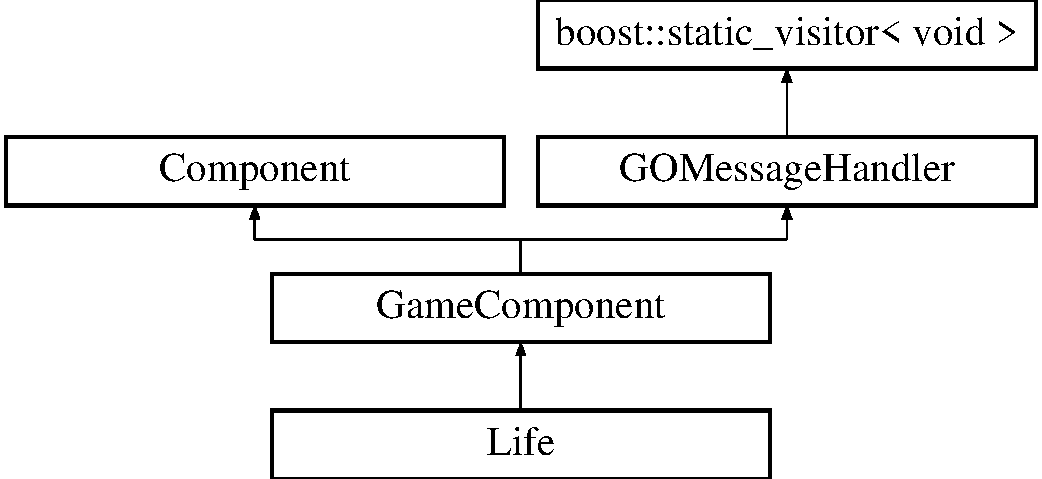
\includegraphics[height=4.000000cm]{class_life}
\end{center}
\end{figure}
\subsection*{Public Member Functions}
\begin{DoxyCompactItemize}
\item 
\hypertarget{class_life_ad5a065168648ef6114eee8851c63a9e0}{}\label{class_life_ad5a065168648ef6114eee8851c63a9e0} 
{\bfseries Life} (\hyperlink{class_game_object}{Game\+Object} $\ast$)
\item 
\hypertarget{class_life_a38250d67d459d3887e8d5adddf6b5129}{}\label{class_life_a38250d67d459d3887e8d5adddf6b5129} 
virtual void {\bfseries init} (int life=1)
\item 
\hypertarget{class_life_a0e00f2735584f3ddebb397742b520d3b}{}\label{class_life_a0e00f2735584f3ddebb397742b520d3b} 
virtual void {\bfseries update} ()
\item 
\hypertarget{class_life_a5058223a20871cf287b7f75ce2eb44ef}{}\label{class_life_a5058223a20871cf287b7f75ce2eb44ef} 
void {\bfseries change\+Life} (int value)
\item 
\hypertarget{class_life_a6bbbcb718407c98ce6c031c81685a659}{}\label{class_life_a6bbbcb718407c98ce6c031c81685a659} 
int {\bfseries get\+Life} ()
\item 
\hypertarget{class_life_ab33e0ff7003ed8c066d61ddb65ffc321}{}\label{class_life_ab33e0ff7003ed8c066d61ddb65ffc321} 
virtual void {\bfseries operator()} (\hyperlink{struct_c_h_a_n_g_e___l_i_f_e}{C\+H\+A\+N\+G\+E\+\_\+\+L\+I\+FE} const \&e)
\end{DoxyCompactItemize}
\subsection*{Protected Attributes}
\begin{DoxyCompactItemize}
\item 
\hypertarget{class_life_a30ed082fad4dd9a0fdf6850ed7b469aa}{}\label{class_life_a30ed082fad4dd9a0fdf6850ed7b469aa} 
int {\bfseries \+\_\+life}
\end{DoxyCompactItemize}
\subsection*{Additional Inherited Members}


The documentation for this class was generated from the following files\+:\begin{DoxyCompactItemize}
\item 
F\+:/\+\_\+\+\_\+\+M\+A\+R\+T\+I\+N/\+\_\+\+\_\+\+E\+N\+J\+M\+I\+N/\+Projets/ascii/shooter/\+A\+S\+C\+I\+I\+\_\+\+S\+H\+O\+O\+T\+E\+R\+\_\+\+P\+R\+O\+T\+O/Life.\+h\item 
F\+:/\+\_\+\+\_\+\+M\+A\+R\+T\+I\+N/\+\_\+\+\_\+\+E\+N\+J\+M\+I\+N/\+Projets/ascii/shooter/\+A\+S\+C\+I\+I\+\_\+\+S\+H\+O\+O\+T\+E\+R\+\_\+\+P\+R\+O\+T\+O/Life.\+cpp\end{DoxyCompactItemize}

\hypertarget{class_movement_component}{}\section{Movement\+Component Class Reference}
\label{class_movement_component}\index{Movement\+Component@{Movement\+Component}}


\hyperlink{class_component}{Component} une velocite.  




{\ttfamily \#include $<$Movement\+Component.\+h$>$}

Inheritance diagram for Movement\+Component\+:\begin{figure}[H]
\begin{center}
\leavevmode
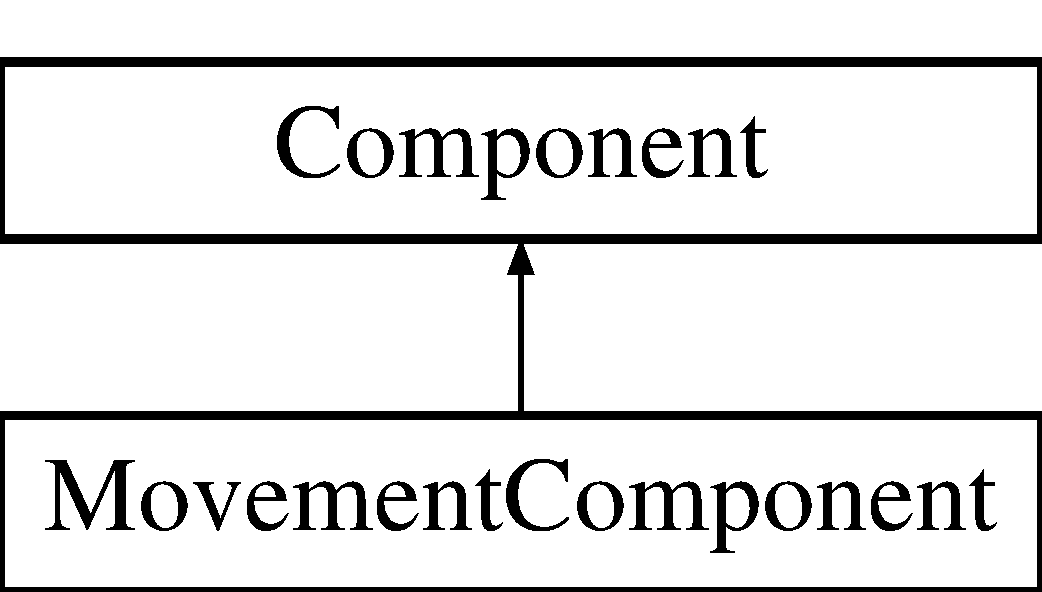
\includegraphics[height=2.000000cm]{class_movement_component}
\end{center}
\end{figure}
\subsection*{Public Member Functions}
\begin{DoxyCompactItemize}
\item 
\hypertarget{class_movement_component_a8c22ac85ae143a750b109a0afcd5832f}{}\label{class_movement_component_a8c22ac85ae143a750b109a0afcd5832f} 
\hyperlink{class_movement_component_a8c22ac85ae143a750b109a0afcd5832f}{Movement\+Component} ()
\begin{DoxyCompactList}\small\item\em Creer un Movement de base de taille (0,0) \end{DoxyCompactList}\item 
\hyperlink{class_movement_component_a2fa2f87c3e4cdc69489e5ce06a131fd1}{Movement\+Component} (float x, float y)
\begin{DoxyCompactList}\small\item\em Creer un Movement de taille (x,y) \end{DoxyCompactList}\item 
\hyperlink{class_movement_component_ac9432753c0b29b1206e04c139e56c757}{Movement\+Component} (\hyperlink{structvector2}{vector2} v)
\begin{DoxyCompactList}\small\item\em Creer un Movement a partir d\textquotesingle{}un \hyperlink{structvector2}{vector2}. \end{DoxyCompactList}\end{DoxyCompactItemize}
\subsection*{Public Attributes}
\begin{DoxyCompactItemize}
\item 
\hypertarget{class_movement_component_aedea2037e7a30160bc7f847055b08088}{}\label{class_movement_component_aedea2037e7a30160bc7f847055b08088} 
\hyperlink{structvector2}{vector2} {\bfseries \+\_\+velocity}
\end{DoxyCompactItemize}


\subsection{Detailed Description}
\hyperlink{class_component}{Component} une velocite. 

\subsection{Constructor \& Destructor Documentation}
\hypertarget{class_movement_component_a2fa2f87c3e4cdc69489e5ce06a131fd1}{}\label{class_movement_component_a2fa2f87c3e4cdc69489e5ce06a131fd1} 
\index{Movement\+Component@{Movement\+Component}!Movement\+Component@{Movement\+Component}}
\index{Movement\+Component@{Movement\+Component}!Movement\+Component@{Movement\+Component}}
\subsubsection{\texorpdfstring{Movement\+Component()}{MovementComponent()}\hspace{0.1cm}{\footnotesize\ttfamily [1/2]}}
{\footnotesize\ttfamily Movement\+Component\+::\+Movement\+Component (\begin{DoxyParamCaption}\item[{float}]{x,  }\item[{float}]{y }\end{DoxyParamCaption})\hspace{0.3cm}{\ttfamily [inline]}}



Creer un Movement de taille (x,y) 


\begin{DoxyParams}{Parameters}
{\em x} & \+: velocite x du Movement \\
\hline
{\em y} & \+: velocite y du Movement \\
\hline
\end{DoxyParams}
\hypertarget{class_movement_component_ac9432753c0b29b1206e04c139e56c757}{}\label{class_movement_component_ac9432753c0b29b1206e04c139e56c757} 
\index{Movement\+Component@{Movement\+Component}!Movement\+Component@{Movement\+Component}}
\index{Movement\+Component@{Movement\+Component}!Movement\+Component@{Movement\+Component}}
\subsubsection{\texorpdfstring{Movement\+Component()}{MovementComponent()}\hspace{0.1cm}{\footnotesize\ttfamily [2/2]}}
{\footnotesize\ttfamily Movement\+Component\+::\+Movement\+Component (\begin{DoxyParamCaption}\item[{\hyperlink{structvector2}{vector2}}]{v }\end{DoxyParamCaption})\hspace{0.3cm}{\ttfamily [inline]}}



Creer un Movement a partir d\textquotesingle{}un \hyperlink{structvector2}{vector2}. 


\begin{DoxyParams}{Parameters}
{\em \hyperlink{structvector2}{vector2}} & qui sera copie dans la velocite du Movement \\
\hline
\end{DoxyParams}


The documentation for this class was generated from the following files\+:\begin{DoxyCompactItemize}
\item 
F\+:/\+\_\+\+\_\+\+M\+A\+R\+T\+I\+N/\+\_\+\+\_\+\+E\+N\+J\+M\+I\+N/\+Projets/ascii/shooter/\+A\+S\+C\+I\+I\+\_\+\+S\+H\+O\+O\+T\+E\+R\+\_\+\+P\+R\+O\+T\+O/Movement\+Component.\+h\item 
F\+:/\+\_\+\+\_\+\+M\+A\+R\+T\+I\+N/\+\_\+\+\_\+\+E\+N\+J\+M\+I\+N/\+Projets/ascii/shooter/\+A\+S\+C\+I\+I\+\_\+\+S\+H\+O\+O\+T\+E\+R\+\_\+\+P\+R\+O\+T\+O/Movement\+Component.\+cpp\end{DoxyCompactItemize}

\hypertarget{class_n_y_timer}{}\section{N\+Y\+Timer Class Reference}
\label{class_n_y_timer}\index{N\+Y\+Timer@{N\+Y\+Timer}}
\subsection*{Public Member Functions}
\begin{DoxyCompactItemize}
\item 
\hypertarget{class_n_y_timer_a3a007c415b8d9c7beafc8e7cefb241f3}{}\label{class_n_y_timer_a3a007c415b8d9c7beafc8e7cefb241f3} 
void {\bfseries start} (void)
\item 
\hypertarget{class_n_y_timer_aa83feb5acbc7baa614b4a434d046aa7d}{}\label{class_n_y_timer_aa83feb5acbc7baa614b4a434d046aa7d} 
float {\bfseries get\+Elapsed\+Seconds} (bool restart=false)
\item 
\hypertarget{class_n_y_timer_abaf8b59d6edbb903fc4869c30787de48}{}\label{class_n_y_timer_abaf8b59d6edbb903fc4869c30787de48} 
unsigned long {\bfseries get\+Elapsed\+Ms} (bool restart=false)
\end{DoxyCompactItemize}
\subsection*{Public Attributes}
\begin{DoxyCompactItemize}
\item 
\hypertarget{class_n_y_timer_a4d8b0b7ff821cb4774f676a4422a9078}{}\label{class_n_y_timer_a4d8b0b7ff821cb4774f676a4422a9078} 
L\+A\+R\+G\+E\+\_\+\+I\+N\+T\+E\+G\+ER {\bfseries last\+Update\+Time}
\item 
\hypertarget{class_n_y_timer_a603b297ae9e287aeb9c4ca410d0fe949}{}\label{class_n_y_timer_a603b297ae9e287aeb9c4ca410d0fe949} 
L\+O\+N\+G\+L\+O\+NG {\bfseries freq}
\end{DoxyCompactItemize}


The documentation for this class was generated from the following file\+:\begin{DoxyCompactItemize}
\item 
F\+:/\+\_\+\+\_\+\+M\+A\+R\+T\+I\+N/\+\_\+\+\_\+\+E\+N\+J\+M\+I\+N/\+Projets/ascii/shooter/\+A\+S\+C\+I\+I\+\_\+\+S\+H\+O\+O\+T\+E\+R\+\_\+\+P\+R\+O\+T\+O/N\+Y\+Timer.\+h\end{DoxyCompactItemize}

\hypertarget{class_physics_engine}{}\section{Physics\+Engine Class Reference}
\label{class_physics_engine}\index{Physics\+Engine@{Physics\+Engine}}
\subsection*{Public Member Functions}
\begin{DoxyCompactItemize}
\item 
\hypertarget{class_physics_engine_a1051e5a80e27864cc8d9c6cfd696c29a}{}\label{class_physics_engine_a1051e5a80e27864cc8d9c6cfd696c29a} 
void {\bfseries init\+Physics} ()
\item 
\hypertarget{class_physics_engine_ac4951e3070893b809ec9b8888ad92e07}{}\label{class_physics_engine_ac4951e3070893b809ec9b8888ad92e07} 
void {\bfseries update} ()
\end{DoxyCompactItemize}


The documentation for this class was generated from the following files\+:\begin{DoxyCompactItemize}
\item 
F\+:/\+\_\+\+\_\+\+M\+A\+R\+T\+I\+N/\+\_\+\+\_\+\+E\+N\+J\+M\+I\+N/\+Projets/ascii/shooter/\+A\+S\+C\+I\+I\+\_\+\+S\+H\+O\+O\+T\+E\+R\+\_\+\+P\+R\+O\+T\+O/Physics\+Engine.\+h\item 
F\+:/\+\_\+\+\_\+\+M\+A\+R\+T\+I\+N/\+\_\+\+\_\+\+E\+N\+J\+M\+I\+N/\+Projets/ascii/shooter/\+A\+S\+C\+I\+I\+\_\+\+S\+H\+O\+O\+T\+E\+R\+\_\+\+P\+R\+O\+T\+O/Physics\+Engine.\+cpp\end{DoxyCompactItemize}

\hypertarget{struct_physics_ignore}{}\section{Physics\+Ignore Struct Reference}
\label{struct_physics_ignore}\index{Physics\+Ignore@{Physics\+Ignore}}
\subsection*{Public Member Functions}
\begin{DoxyCompactItemize}
\item 
\hypertarget{struct_physics_ignore_a4992567e145c907dc22e9594fdac4c84}{}\label{struct_physics_ignore_a4992567e145c907dc22e9594fdac4c84} 
bool {\bfseries ignore} (string t1, string t2)
\end{DoxyCompactItemize}
\subsection*{Public Attributes}
\begin{DoxyCompactItemize}
\item 
\hypertarget{struct_physics_ignore_a8c2d4c55ba67b5c4d5c97a97ca815553}{}\label{struct_physics_ignore_a8c2d4c55ba67b5c4d5c97a97ca815553} 
string {\bfseries tag1}
\item 
\hypertarget{struct_physics_ignore_ab951c2347a6c7442ee1baa820330d299}{}\label{struct_physics_ignore_ab951c2347a6c7442ee1baa820330d299} 
string {\bfseries tag2}
\end{DoxyCompactItemize}


The documentation for this struct was generated from the following file\+:\begin{DoxyCompactItemize}
\item 
F\+:/\+\_\+\+\_\+\+M\+A\+R\+T\+I\+N/\+\_\+\+\_\+\+E\+N\+J\+M\+I\+N/\+Projets/ascii/shooter/\+A\+S\+C\+I\+I\+\_\+\+S\+H\+O\+O\+T\+E\+R\+\_\+\+P\+R\+O\+T\+O/Structures.\+h\end{DoxyCompactItemize}

\hypertarget{structpixel}{}\section{pixel Struct Reference}
\label{structpixel}\index{pixel@{pixel}}
\subsection*{Public Attributes}
\begin{DoxyCompactItemize}
\item 
\hypertarget{structpixel_a9e2448882ee65d100d7f0d829cce90f5}{}\label{structpixel_a9e2448882ee65d100d7f0d829cce90f5} 
C\+H\+A\+R\+\_\+\+I\+N\+FO {\bfseries c}
\item 
\hypertarget{structpixel_abab54e3f587bb32bd669539eafb199f5}{}\label{structpixel_abab54e3f587bb32bd669539eafb199f5} 
int {\bfseries x}
\item 
\hypertarget{structpixel_ac8ce17202b68b5efe159e68c0fed89e9}{}\label{structpixel_ac8ce17202b68b5efe159e68c0fed89e9} 
int {\bfseries y}
\end{DoxyCompactItemize}


The documentation for this struct was generated from the following file\+:\begin{DoxyCompactItemize}
\item 
F\+:/\+\_\+\+\_\+\+M\+A\+R\+T\+I\+N/\+\_\+\+\_\+\+E\+N\+J\+M\+I\+N/\+Projets/ascii/shooter/\+A\+S\+C\+I\+I\+\_\+\+S\+H\+O\+O\+T\+E\+R\+\_\+\+P\+R\+O\+T\+O/Structures.\+h\end{DoxyCompactItemize}

\hypertarget{class_player}{}\section{Player Class Reference}
\label{class_player}\index{Player@{Player}}
Inheritance diagram for Player\+:\begin{figure}[H]
\begin{center}
\leavevmode
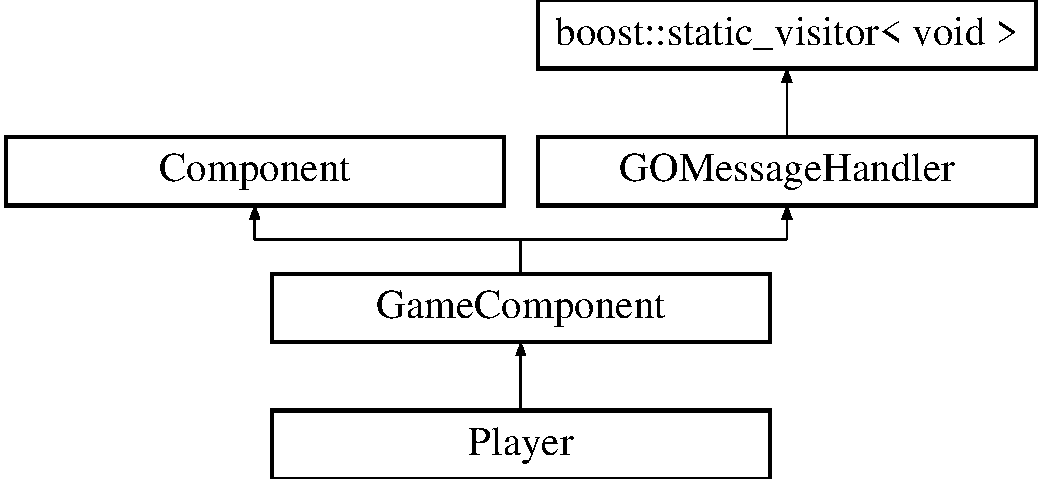
\includegraphics[height=4.000000cm]{class_player}
\end{center}
\end{figure}
\subsection*{Public Member Functions}
\begin{DoxyCompactItemize}
\item 
\hypertarget{class_player_ac9e2313c9f0599f111d51b1ededc7b59}{}\label{class_player_ac9e2313c9f0599f111d51b1ededc7b59} 
{\bfseries Player} (\hyperlink{class_game_object}{Game\+Object} $\ast$g)
\item 
\hypertarget{class_player_abde7e5d5c9b248e9d151b63342a1651f}{}\label{class_player_abde7e5d5c9b248e9d151b63342a1651f} 
virtual void {\bfseries init} (int life=5, std\+::string path=\char`\"{}Ship1.\+txt\char`\"{}, float speed=20, float fire\+Rate=100.\+0)
\item 
\hypertarget{class_player_a82c3476f3e65a4e2ac6bcd040771bdd4}{}\label{class_player_a82c3476f3e65a4e2ac6bcd040771bdd4} 
virtual void {\bfseries update} ()
\end{DoxyCompactItemize}
\subsection*{Protected Member Functions}
\begin{DoxyCompactItemize}
\item 
\hypertarget{class_player_a404b1d420a802000bdca0ac07f463c9b}{}\label{class_player_a404b1d420a802000bdca0ac07f463c9b} 
void {\bfseries init\+Values} (float speed, float fire\+Rate)
\item 
\hypertarget{class_player_a505efa3aa6fa4e21a84200399cc90f4d}{}\label{class_player_a505efa3aa6fa4e21a84200399cc90f4d} 
void {\bfseries init\+Component} (int life, std\+::string path)
\item 
\hypertarget{class_player_ae02ee46d8c20dd0697b975f935b09839}{}\label{class_player_ae02ee46d8c20dd0697b975f935b09839} 
void {\bfseries move} ()
\item 
\hypertarget{class_player_a5dc98bda088b0e253956ef22eba154f0}{}\label{class_player_a5dc98bda088b0e253956ef22eba154f0} 
void {\bfseries fire} ()
\item 
\hypertarget{class_player_ac4c7b097b1e703f026c80a1142648fbd}{}\label{class_player_ac4c7b097b1e703f026c80a1142648fbd} 
void {\bfseries update\+Time} ()
\item 
\hypertarget{class_player_ae4b66b26311d3a7f2fe5b35edfe6e97a}{}\label{class_player_ae4b66b26311d3a7f2fe5b35edfe6e97a} 
void {\bfseries fire1} ()
\item 
\hypertarget{class_player_ad03f605930d87fecefaf5f07972c8514}{}\label{class_player_ad03f605930d87fecefaf5f07972c8514} 
void {\bfseries fire2} ()
\end{DoxyCompactItemize}
\subsection*{Protected Attributes}
\begin{DoxyCompactItemize}
\item 
\hypertarget{class_player_a2058005a9cb8d0ee1930178ab5965ac1}{}\label{class_player_a2058005a9cb8d0ee1930178ab5965ac1} 
float {\bfseries \+\_\+speed}
\item 
\hypertarget{class_player_ac242a65fa0bd42e9eb38782c214eb616}{}\label{class_player_ac242a65fa0bd42e9eb38782c214eb616} 
\hyperlink{class_n_y_timer}{N\+Y\+Timer} $\ast$ {\bfseries \+\_\+timer}
\item 
\hypertarget{class_player_a275c2f72e87a8adbac297ff39171a29f}{}\label{class_player_a275c2f72e87a8adbac297ff39171a29f} 
double {\bfseries \+\_\+fire\+Rate1}
\item 
\hypertarget{class_player_aee9448eeba5e2c13c69d7c02846027f6}{}\label{class_player_aee9448eeba5e2c13c69d7c02846027f6} 
double {\bfseries \+\_\+previous1}
\item 
\hypertarget{class_player_a2d253a3b9a3cfed734009bc9f0e279e7}{}\label{class_player_a2d253a3b9a3cfed734009bc9f0e279e7} 
double {\bfseries \+\_\+elapsed1}
\item 
\hypertarget{class_player_a5da7f87d45d122ce555a96848a60df91}{}\label{class_player_a5da7f87d45d122ce555a96848a60df91} 
double {\bfseries \+\_\+fire\+Rate2}
\item 
\hypertarget{class_player_aff92a376478133301307cf8701ac8281}{}\label{class_player_aff92a376478133301307cf8701ac8281} 
double {\bfseries \+\_\+previous2}
\item 
\hypertarget{class_player_a407fc2edf69c09187c1f2b9ac1bb9310}{}\label{class_player_a407fc2edf69c09187c1f2b9ac1bb9310} 
double {\bfseries \+\_\+elapsed2}
\end{DoxyCompactItemize}


The documentation for this class was generated from the following files\+:\begin{DoxyCompactItemize}
\item 
F\+:/\+\_\+\+\_\+\+M\+A\+R\+T\+I\+N/\+\_\+\+\_\+\+E\+N\+J\+M\+I\+N/\+Projets/ascii/shooter/\+A\+S\+C\+I\+I\+\_\+\+S\+H\+O\+O\+T\+E\+R\+\_\+\+P\+R\+O\+T\+O/Player.\+h\item 
F\+:/\+\_\+\+\_\+\+M\+A\+R\+T\+I\+N/\+\_\+\+\_\+\+E\+N\+J\+M\+I\+N/\+Projets/ascii/shooter/\+A\+S\+C\+I\+I\+\_\+\+S\+H\+O\+O\+T\+E\+R\+\_\+\+P\+R\+O\+T\+O/Player.\+cpp\end{DoxyCompactItemize}

\hypertarget{class_rocket}{}\section{Rocket Class Reference}
\label{class_rocket}\index{Rocket@{Rocket}}
Inheritance diagram for Rocket\+:\begin{figure}[H]
\begin{center}
\leavevmode
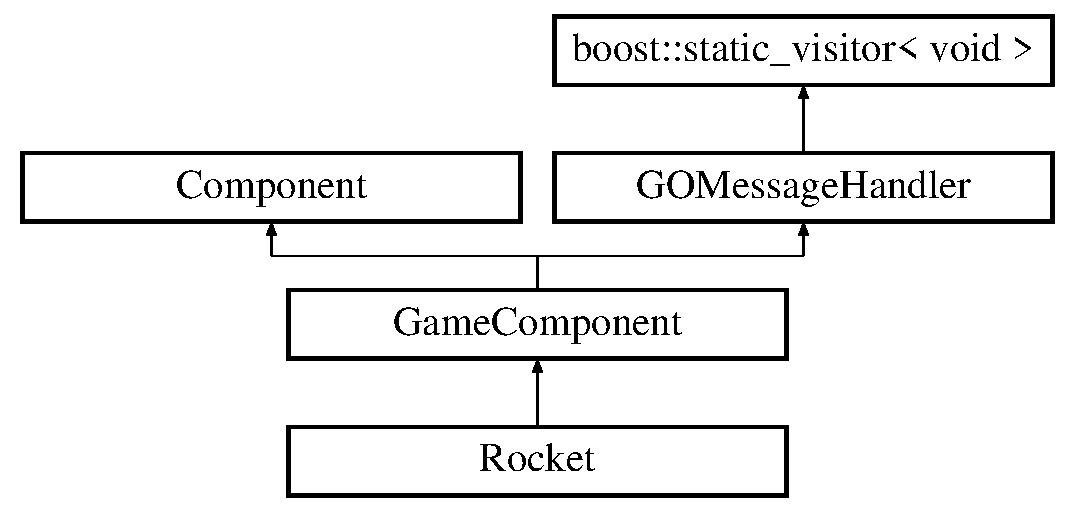
\includegraphics[height=4.000000cm]{class_rocket}
\end{center}
\end{figure}
\subsection*{Public Member Functions}
\begin{DoxyCompactItemize}
\item 
\hyperlink{class_rocket_aa1ab185c1ec59b4983114b41efd59ea0}{Rocket} (\hyperlink{class_game_object}{Game\+Object} $\ast$)
\item 
void \hyperlink{class_rocket_ace1889a9c70f40bafb955dbc48ecc9d0}{init} (int life=1, \hyperlink{structvector2}{vector2} velocity=\{ 1, 0 \}, float speed=6.\+0)
\begin{DoxyCompactList}\small\item\em initialise le joueur avec les valeurs necessaires \end{DoxyCompactList}\item 
virtual void \hyperlink{class_rocket_aa0f4dcf673358e841e4b4b2fa0b1462e}{update} ()
\end{DoxyCompactItemize}
\subsection*{Protected Member Functions}
\begin{DoxyCompactItemize}
\item 
\hypertarget{class_rocket_aa73e743c57e1be5dd4c23c3dc5bc498f}{}\label{class_rocket_aa73e743c57e1be5dd4c23c3dc5bc498f} 
void {\bfseries init\+Values} (float speed)
\item 
\hypertarget{class_rocket_a3f444dd351e952656067724b1fc7b1ee}{}\label{class_rocket_a3f444dd351e952656067724b1fc7b1ee} 
void {\bfseries init\+Component} (int life, \hyperlink{structvector2}{vector2} velocity)
\item 
\hypertarget{class_rocket_aa9131c195e7b644b036f745df9b00e94}{}\label{class_rocket_aa9131c195e7b644b036f745df9b00e94} 
void {\bfseries move} ()
\end{DoxyCompactItemize}
\subsection*{Protected Attributes}
\begin{DoxyCompactItemize}
\item 
\hypertarget{class_rocket_aa0c252aa8094bc942d743aed643fcf08}{}\label{class_rocket_aa0c252aa8094bc942d743aed643fcf08} 
float {\bfseries \+\_\+speed}
\end{DoxyCompactItemize}


\subsection{Constructor \& Destructor Documentation}
\hypertarget{class_rocket_aa1ab185c1ec59b4983114b41efd59ea0}{}\label{class_rocket_aa1ab185c1ec59b4983114b41efd59ea0} 
\index{Rocket@{Rocket}!Rocket@{Rocket}}
\index{Rocket@{Rocket}!Rocket@{Rocket}}
\subsubsection{\texorpdfstring{Rocket()}{Rocket()}}
{\footnotesize\ttfamily Rocket\+::\+Rocket (\begin{DoxyParamCaption}\item[{\hyperlink{class_game_object}{Game\+Object} $\ast$}]{obj }\end{DoxyParamCaption})}

cf. constructeur de \hyperlink{class_game_component}{Game\+Component} 

\subsection{Member Function Documentation}
\hypertarget{class_rocket_ace1889a9c70f40bafb955dbc48ecc9d0}{}\label{class_rocket_ace1889a9c70f40bafb955dbc48ecc9d0} 
\index{Rocket@{Rocket}!init@{init}}
\index{init@{init}!Rocket@{Rocket}}
\subsubsection{\texorpdfstring{init()}{init()}}
{\footnotesize\ttfamily void Rocket\+::init (\begin{DoxyParamCaption}\item[{int}]{life = {\ttfamily 1},  }\item[{\hyperlink{structvector2}{vector2}}]{velocity = {\ttfamily \{~1,~0~\}},  }\item[{float}]{speed = {\ttfamily 6.0} }\end{DoxyParamCaption})}



initialise le joueur avec les valeurs necessaires 


\begin{DoxyParams}{Parameters}
{\em vie} & initiale du missile \\
\hline
{\em vitesse} & initiale du joueur \\
\hline
{\em fire} & rate du joueur \\
\hline
\end{DoxyParams}
\hypertarget{class_rocket_aa0f4dcf673358e841e4b4b2fa0b1462e}{}\label{class_rocket_aa0f4dcf673358e841e4b4b2fa0b1462e} 
\index{Rocket@{Rocket}!update@{update}}
\index{update@{update}!Rocket@{Rocket}}
\subsubsection{\texorpdfstring{update()}{update()}}
{\footnotesize\ttfamily void Rocket\+::update (\begin{DoxyParamCaption}{ }\end{DoxyParamCaption})\hspace{0.3cm}{\ttfamily [virtual]}}

la position du missile 

Implements \hyperlink{class_game_component_a65fc004cd4dc7593052327ff874bb2f0}{Game\+Component}.



The documentation for this class was generated from the following files\+:\begin{DoxyCompactItemize}
\item 
F\+:/\+\_\+\+\_\+\+M\+A\+R\+T\+I\+N/\+\_\+\+\_\+\+E\+N\+J\+M\+I\+N/\+Projets/ascii/shooter/\+A\+S\+C\+I\+I\+\_\+\+S\+H\+O\+O\+T\+E\+R\+\_\+\+P\+R\+O\+T\+O/Rocket.\+h\item 
F\+:/\+\_\+\+\_\+\+M\+A\+R\+T\+I\+N/\+\_\+\+\_\+\+E\+N\+J\+M\+I\+N/\+Projets/ascii/shooter/\+A\+S\+C\+I\+I\+\_\+\+S\+H\+O\+O\+T\+E\+R\+\_\+\+P\+R\+O\+T\+O/Rocket.\+cpp\end{DoxyCompactItemize}

\hypertarget{class_scene}{}\section{Scene Class Reference}
\label{class_scene}\index{Scene@{Scene}}


Classe gerant une scene, c\textquotesingle{}est a dire une liste de \hyperlink{class_game_object}{Game\+Object}.  




{\ttfamily \#include $<$Scene.\+h$>$}

\subsection*{Public Member Functions}
\begin{DoxyCompactItemize}
\item 
\hypertarget{class_scene_a6fb788d6ae25d5293d3a58966cf29757}{}\label{class_scene_a6fb788d6ae25d5293d3a58966cf29757} 
{\bfseries Scene} (std\+::string name)
\item 
\hypertarget{class_scene_abb3b6efc6fdba03cd96436edaf08a967}{}\label{class_scene_abb3b6efc6fdba03cd96436edaf08a967} 
void \hyperlink{class_scene_abb3b6efc6fdba03cd96436edaf08a967}{init} ()
\begin{DoxyCompactList}\small\item\em Initialise la scene. \end{DoxyCompactList}\item 
\hypertarget{class_scene_aa24c7e636c10e4e42650c1374b90bb80}{}\label{class_scene_aa24c7e636c10e4e42650c1374b90bb80} 
void \hyperlink{class_scene_aa24c7e636c10e4e42650c1374b90bb80}{update} ()
\begin{DoxyCompactList}\small\item\em Update tous les \hyperlink{class_game_object}{Game\+Object} possedes par la scene. \end{DoxyCompactList}\item 
\hypertarget{class_scene_a70e5b1218abb729d70d9f41b107017f9}{}\label{class_scene_a70e5b1218abb729d70d9f41b107017f9} 
void \hyperlink{class_scene_a70e5b1218abb729d70d9f41b107017f9}{clear} ()
\begin{DoxyCompactList}\small\item\em Supprime les \hyperlink{class_game_object}{Game\+Object} de la scene. \end{DoxyCompactList}\item 
\hypertarget{class_scene_a95d3218f52081eea9e34d2d2bdff94df}{}\label{class_scene_a95d3218f52081eea9e34d2d2bdff94df} 
void \hyperlink{class_scene_a95d3218f52081eea9e34d2d2bdff94df}{take\+Care\+Of\+Dead\+Bodies} ()
\begin{DoxyCompactList}\small\item\em Supprime tous les \hyperlink{class_game_object}{Game\+Object} morts lors de l\textquotesingle{}update precedant. \end{DoxyCompactList}\item 
void \hyperlink{class_scene_aed7c3cfbef1cfa439af13e56dfd5a07c}{add\+Object} (\hyperlink{class_game_object}{Game\+Object} $\ast$)
\begin{DoxyCompactList}\small\item\em Ajout un \hyperlink{class_game_object}{Game\+Object} a la scene. \end{DoxyCompactList}\item 
void \hyperlink{class_scene_a9058ae3eed897e4e18f977abfd53e348}{remove\+Object} (\hyperlink{class_game_object}{Game\+Object} $\ast$)
\begin{DoxyCompactList}\small\item\em Supprime un \hyperlink{class_game_object}{Game\+Object} a la scene. \end{DoxyCompactList}\item 
std\+::vector$<$ \hyperlink{class_game_object}{Game\+Object} $\ast$ $>$ \& \hyperlink{class_scene_a9e7d39e9d4b1d6b76997e1453738658d}{get\+Objects} ()
\begin{DoxyCompactList}\small\item\em Permet d\textquotesingle{}acceder aux \hyperlink{class_game_object}{Game\+Object} de la \hyperlink{class_scene}{Scene}. \end{DoxyCompactList}\item 
void \hyperlink{class_scene_a75722f5960b037b0ec6d9cdf04ff9fa1}{send\+G\+O\+Message} (const G\+O\+Message) const
\begin{DoxyCompactList}\small\item\em Envoie un G\+O\+Message a tous les \hyperlink{class_game_object}{Game\+Object} de la \hyperlink{class_scene}{Scene}. \end{DoxyCompactList}\end{DoxyCompactItemize}
\subsection*{Public Attributes}
\begin{DoxyCompactItemize}
\item 
\hypertarget{class_scene_afbb5064e07cb2904ecd2cfb0096a00c9}{}\label{class_scene_afbb5064e07cb2904ecd2cfb0096a00c9} 
std\+::string \hyperlink{class_scene_afbb5064e07cb2904ecd2cfb0096a00c9}{\+\_\+name}
\begin{DoxyCompactList}\small\item\em Le nom de la \hyperlink{class_scene}{Scene}. \end{DoxyCompactList}\end{DoxyCompactItemize}
\subsection*{Protected Attributes}
\begin{DoxyCompactItemize}
\item 
\hypertarget{class_scene_a08d7cc1bd05adcaedf8d264c8b9a3da2}{}\label{class_scene_a08d7cc1bd05adcaedf8d264c8b9a3da2} 
std\+::vector$<$ \hyperlink{class_game_object}{Game\+Object} $\ast$ $>$ {\bfseries \+\_\+objects}
\end{DoxyCompactItemize}


\subsection{Detailed Description}
Classe gerant une scene, c\textquotesingle{}est a dire une liste de \hyperlink{class_game_object}{Game\+Object}. 

\subsection{Member Function Documentation}
\hypertarget{class_scene_aed7c3cfbef1cfa439af13e56dfd5a07c}{}\label{class_scene_aed7c3cfbef1cfa439af13e56dfd5a07c} 
\index{Scene@{Scene}!add\+Object@{add\+Object}}
\index{add\+Object@{add\+Object}!Scene@{Scene}}
\subsubsection{\texorpdfstring{add\+Object()}{addObject()}}
{\footnotesize\ttfamily void Scene\+::add\+Object (\begin{DoxyParamCaption}\item[{\hyperlink{class_game_object}{Game\+Object} $\ast$}]{obj }\end{DoxyParamCaption})}



Ajout un \hyperlink{class_game_object}{Game\+Object} a la scene. 


\begin{DoxyParams}{Parameters}
{\em Le} & \hyperlink{class_game_object}{Game\+Object} a ajouter \\
\hline
\end{DoxyParams}
\hypertarget{class_scene_a9e7d39e9d4b1d6b76997e1453738658d}{}\label{class_scene_a9e7d39e9d4b1d6b76997e1453738658d} 
\index{Scene@{Scene}!get\+Objects@{get\+Objects}}
\index{get\+Objects@{get\+Objects}!Scene@{Scene}}
\subsubsection{\texorpdfstring{get\+Objects()}{getObjects()}}
{\footnotesize\ttfamily vector$<$ \hyperlink{class_game_object}{Game\+Object} $\ast$ $>$ \& Scene\+::get\+Objects (\begin{DoxyParamCaption}{ }\end{DoxyParamCaption})}



Permet d\textquotesingle{}acceder aux \hyperlink{class_game_object}{Game\+Object} de la \hyperlink{class_scene}{Scene}. 

\begin{DoxyReturn}{Returns}
Les Game\+Objects possedes par la \hyperlink{class_scene}{Scene} 
\end{DoxyReturn}
\hypertarget{class_scene_a9058ae3eed897e4e18f977abfd53e348}{}\label{class_scene_a9058ae3eed897e4e18f977abfd53e348} 
\index{Scene@{Scene}!remove\+Object@{remove\+Object}}
\index{remove\+Object@{remove\+Object}!Scene@{Scene}}
\subsubsection{\texorpdfstring{remove\+Object()}{removeObject()}}
{\footnotesize\ttfamily void Scene\+::remove\+Object (\begin{DoxyParamCaption}\item[{\hyperlink{class_game_object}{Game\+Object} $\ast$}]{obj }\end{DoxyParamCaption})}



Supprime un \hyperlink{class_game_object}{Game\+Object} a la scene. 


\begin{DoxyParams}{Parameters}
{\em Le} & \hyperlink{class_game_object}{Game\+Object} a supprimer \\
\hline
\end{DoxyParams}
\hypertarget{class_scene_a75722f5960b037b0ec6d9cdf04ff9fa1}{}\label{class_scene_a75722f5960b037b0ec6d9cdf04ff9fa1} 
\index{Scene@{Scene}!send\+G\+O\+Message@{send\+G\+O\+Message}}
\index{send\+G\+O\+Message@{send\+G\+O\+Message}!Scene@{Scene}}
\subsubsection{\texorpdfstring{send\+G\+O\+Message()}{sendGOMessage()}}
{\footnotesize\ttfamily void Scene\+::send\+G\+O\+Message (\begin{DoxyParamCaption}\item[{const G\+O\+Message}]{message }\end{DoxyParamCaption}) const}



Envoie un G\+O\+Message a tous les \hyperlink{class_game_object}{Game\+Object} de la \hyperlink{class_scene}{Scene}. 


\begin{DoxyParams}{Parameters}
{\em Le} & G\+O\+Message a envoyer \\
\hline
\end{DoxyParams}


The documentation for this class was generated from the following files\+:\begin{DoxyCompactItemize}
\item 
F\+:/\+\_\+\+\_\+\+M\+A\+R\+T\+I\+N/\+\_\+\+\_\+\+E\+N\+J\+M\+I\+N/\+Projets/ascii/shooter/\+A\+S\+C\+I\+I\+\_\+\+S\+H\+O\+O\+T\+E\+R\+\_\+\+P\+R\+O\+T\+O/Scene.\+h\item 
F\+:/\+\_\+\+\_\+\+M\+A\+R\+T\+I\+N/\+\_\+\+\_\+\+E\+N\+J\+M\+I\+N/\+Projets/ascii/shooter/\+A\+S\+C\+I\+I\+\_\+\+S\+H\+O\+O\+T\+E\+R\+\_\+\+P\+R\+O\+T\+O/Scene.\+cpp\end{DoxyCompactItemize}

\hypertarget{class_s_c_message_handler}{}\section{S\+C\+Message\+Handler Class Reference}
\label{class_s_c_message_handler}\index{S\+C\+Message\+Handler@{S\+C\+Message\+Handler}}
Inheritance diagram for S\+C\+Message\+Handler\+:\begin{figure}[H]
\begin{center}
\leavevmode
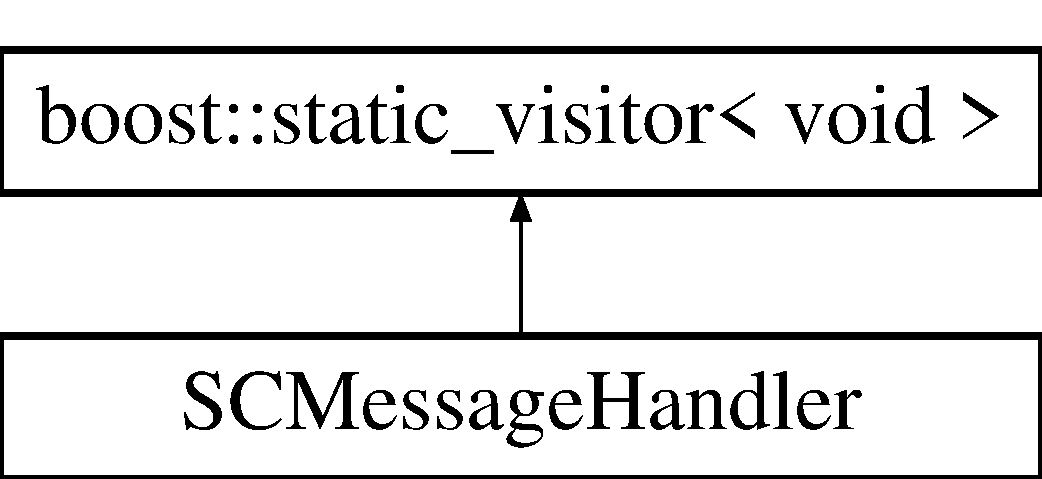
\includegraphics[height=2.000000cm]{class_s_c_message_handler}
\end{center}
\end{figure}
\subsection*{Public Member Functions}
\begin{DoxyCompactItemize}
\item 
\hypertarget{class_s_c_message_handler_a8c8eb5ee23f04dbf644c5f4715d80b5e}{}\label{class_s_c_message_handler_a8c8eb5ee23f04dbf644c5f4715d80b5e} 
virtual void {\bfseries operator()} (\hyperlink{struct_d_e_s_t_r_o_y}{D\+E\+S\+T\+R\+OY} const \&e)
\end{DoxyCompactItemize}


The documentation for this class was generated from the following files\+:\begin{DoxyCompactItemize}
\item 
F\+:/\+\_\+\+\_\+\+M\+A\+R\+T\+I\+N/\+\_\+\+\_\+\+E\+N\+J\+M\+I\+N/\+Projets/ascii/shooter/\+A\+S\+C\+I\+I\+\_\+\+S\+H\+O\+O\+T\+E\+R\+\_\+\+P\+R\+O\+T\+O/Message\+Handler.\+h\item 
F\+:/\+\_\+\+\_\+\+M\+A\+R\+T\+I\+N/\+\_\+\+\_\+\+E\+N\+J\+M\+I\+N/\+Projets/ascii/shooter/\+A\+S\+C\+I\+I\+\_\+\+S\+H\+O\+O\+T\+E\+R\+\_\+\+P\+R\+O\+T\+O/Message\+Handler.\+cpp\end{DoxyCompactItemize}

\hypertarget{class_u_i}{}\section{UI Class Reference}
\label{class_u_i}\index{UI@{UI}}
Inheritance diagram for UI\+:\begin{figure}[H]
\begin{center}
\leavevmode
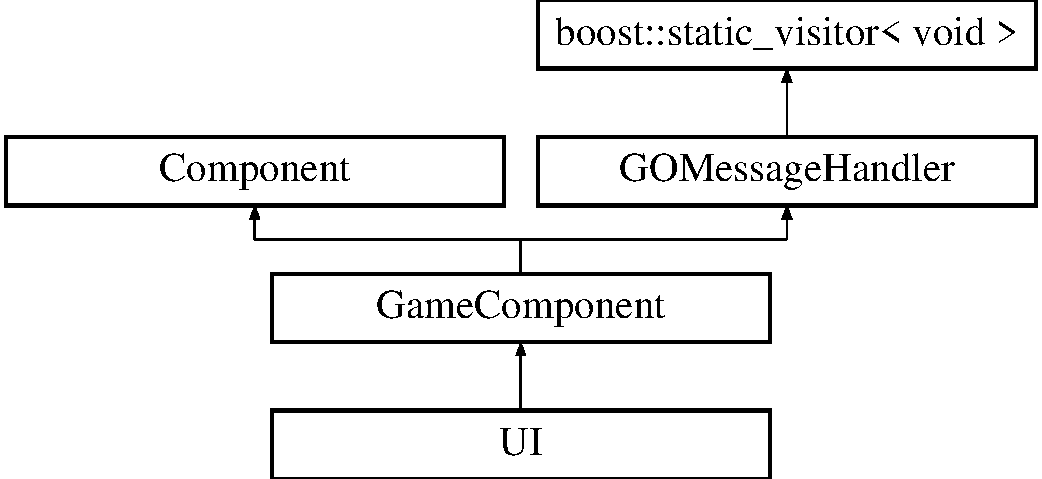
\includegraphics[height=4.000000cm]{class_u_i}
\end{center}
\end{figure}
\subsection*{Public Member Functions}
\begin{DoxyCompactItemize}
\item 
\hyperlink{class_u_i_ab299e77b21896655f94ef84c727a4e22}{UI} (\hyperlink{class_game_object}{Game\+Object} $\ast$)
\item 
\hypertarget{class_u_i_a2277decc2cba013de2fbb5a64fbc1543}{}\label{class_u_i_a2277decc2cba013de2fbb5a64fbc1543} 
virtual void \hyperlink{class_u_i_a2277decc2cba013de2fbb5a64fbc1543}{init} ()
\begin{DoxyCompactList}\small\item\em Initialise le \hyperlink{class_game_component}{Game\+Component}. \end{DoxyCompactList}\item 
\hypertarget{class_u_i_a47c96192a9924bbd6c6b610922770988}{}\label{class_u_i_a47c96192a9924bbd6c6b610922770988} 
virtual void \hyperlink{class_u_i_a47c96192a9924bbd6c6b610922770988}{update} ()
\begin{DoxyCompactList}\small\item\em Update le \hyperlink{class_game_component}{Game\+Component} a chaque tick. \end{DoxyCompactList}\item 
\hypertarget{class_u_i_ae16be0e89513445e6a75e7cd92ba6d90}{}\label{class_u_i_ae16be0e89513445e6a75e7cd92ba6d90} 
virtual void \hyperlink{class_u_i_ae16be0e89513445e6a75e7cd92ba6d90}{wake} ()
\begin{DoxyCompactList}\small\item\em Reset le \hyperlink{class_game_component}{Game\+Component}. \end{DoxyCompactList}\item 
\hypertarget{class_u_i_a103e73ecc7a0e62c01d1c21f5bcc0fe7}{}\label{class_u_i_a103e73ecc7a0e62c01d1c21f5bcc0fe7} 
void {\bfseries set\+Context} (\hyperlink{struct_u_i_c_o_n_t_e_x_t}{U\+I\+C\+O\+N\+T\+E\+XT} const \&context)
\item 
\hypertarget{class_u_i_a7a1beee6c64d0fce1f6e4dc720b08ea3}{}\label{class_u_i_a7a1beee6c64d0fce1f6e4dc720b08ea3} 
virtual void {\bfseries operator()} (\hyperlink{struct_u_i_c_o_n_t_e_x_t}{U\+I\+C\+O\+N\+T\+E\+XT} const \&e)
\end{DoxyCompactItemize}
\subsection*{Protected Member Functions}
\begin{DoxyCompactItemize}
\item 
\hypertarget{class_u_i_a2f93274796ee43d83145b042b1844b93}{}\label{class_u_i_a2f93274796ee43d83145b042b1844b93} 
void {\bfseries set\+Graphics} ()
\item 
\hypertarget{class_u_i_a626a653f29b66e351efe58085001ad87}{}\label{class_u_i_a626a653f29b66e351efe58085001ad87} 
void {\bfseries set\+Bullet\+Positions} ()
\end{DoxyCompactItemize}
\subsection*{Protected Attributes}
\begin{DoxyCompactItemize}
\item 
\hypertarget{class_u_i_aac95c488322f728b500db6d6b2c57ec4}{}\label{class_u_i_aac95c488322f728b500db6d6b2c57ec4} 
\hyperlink{class_u_i_bullet}{U\+I\+Bullet} $\ast$ {\bfseries \+\_\+ui\+Bullet}
\item 
\hypertarget{class_u_i_a6c660cea67e5c6f8c2e94a6f218e5589}{}\label{class_u_i_a6c660cea67e5c6f8c2e94a6f218e5589} 
\hyperlink{struct_u_i_c_o_n_t_e_x_t}{U\+I\+C\+O\+N\+T\+E\+XT} {\bfseries \+\_\+context}
\item 
\hypertarget{class_u_i_ad27cd3cd68f3ab9f8626dc855891ec39}{}\label{class_u_i_ad27cd3cd68f3ab9f8626dc855891ec39} 
\hyperlink{class_graphics_component}{Graphics\+Component} $\ast$ {\bfseries \+\_\+graphics}
\end{DoxyCompactItemize}


\subsection{Constructor \& Destructor Documentation}
\hypertarget{class_u_i_ab299e77b21896655f94ef84c727a4e22}{}\label{class_u_i_ab299e77b21896655f94ef84c727a4e22} 
\index{UI@{UI}!UI@{UI}}
\index{UI@{UI}!UI@{UI}}
\subsubsection{\texorpdfstring{U\+I()}{UI()}}
{\footnotesize\ttfamily U\+I\+::\+UI (\begin{DoxyParamCaption}\item[{\hyperlink{class_game_object}{Game\+Object} $\ast$}]{obj }\end{DoxyParamCaption})}

cf. constructeur de \hyperlink{class_game_component}{Game\+Component} 

The documentation for this class was generated from the following files\+:\begin{DoxyCompactItemize}
\item 
F\+:/\+\_\+\+\_\+\+M\+A\+R\+T\+I\+N/\+\_\+\+\_\+\+E\+N\+J\+M\+I\+N/\+Projets/ascii/shooter/\+A\+S\+C\+I\+I\+\_\+\+S\+H\+O\+O\+T\+E\+R\+\_\+\+P\+R\+O\+T\+O/U\+I.\+h\item 
F\+:/\+\_\+\+\_\+\+M\+A\+R\+T\+I\+N/\+\_\+\+\_\+\+E\+N\+J\+M\+I\+N/\+Projets/ascii/shooter/\+A\+S\+C\+I\+I\+\_\+\+S\+H\+O\+O\+T\+E\+R\+\_\+\+P\+R\+O\+T\+O/U\+I.\+cpp\end{DoxyCompactItemize}

\hypertarget{class_u_i_bullet}{}\section{U\+I\+Bullet Class Reference}
\label{class_u_i_bullet}\index{U\+I\+Bullet@{U\+I\+Bullet}}
Inheritance diagram for U\+I\+Bullet\+:\begin{figure}[H]
\begin{center}
\leavevmode
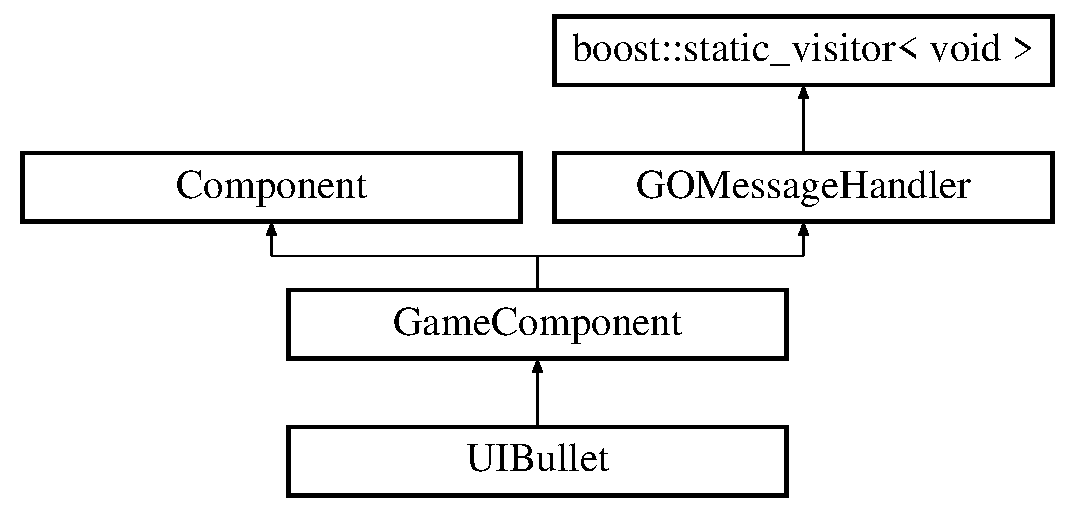
\includegraphics[height=4.000000cm]{class_u_i_bullet}
\end{center}
\end{figure}
\subsection*{Public Member Functions}
\begin{DoxyCompactItemize}
\item 
\hyperlink{class_u_i_bullet_a5036f0f1649cbb182b46a37ba4096bc1}{U\+I\+Bullet} (\hyperlink{class_game_object}{Game\+Object} $\ast$)
\item 
\hypertarget{class_u_i_bullet_a46d657568a2458cbf6206265e17f966b}{}\label{class_u_i_bullet_a46d657568a2458cbf6206265e17f966b} 
virtual void \hyperlink{class_u_i_bullet_a46d657568a2458cbf6206265e17f966b}{init} ()
\begin{DoxyCompactList}\small\item\em Initialise le \hyperlink{class_game_component}{Game\+Component}. \end{DoxyCompactList}\item 
\hypertarget{class_u_i_bullet_ad88e53627d06397907b9537c809626ed}{}\label{class_u_i_bullet_ad88e53627d06397907b9537c809626ed} 
virtual void \hyperlink{class_u_i_bullet_ad88e53627d06397907b9537c809626ed}{update} ()
\begin{DoxyCompactList}\small\item\em Update le \hyperlink{class_game_component}{Game\+Component} a chaque tick. \end{DoxyCompactList}\item 
\hypertarget{class_u_i_bullet_a92bc30d8dc5a23773e0a12ff92d400ae}{}\label{class_u_i_bullet_a92bc30d8dc5a23773e0a12ff92d400ae} 
void {\bfseries set\+Context} (\hyperlink{struct_u_i_c_o_n_t_e_x_t}{U\+I\+C\+O\+N\+T\+E\+XT} context)
\end{DoxyCompactItemize}
\subsection*{Protected Attributes}
\begin{DoxyCompactItemize}
\item 
\hypertarget{class_u_i_bullet_a75026bf852c57c18b5b4147cd65b1569}{}\label{class_u_i_bullet_a75026bf852c57c18b5b4147cd65b1569} 
\hyperlink{class_u_i}{UI} $\ast$ {\bfseries \+\_\+ui}
\item 
\hypertarget{class_u_i_bullet_a40405d6b8e46afab0e80e492d18a7605}{}\label{class_u_i_bullet_a40405d6b8e46afab0e80e492d18a7605} 
\hyperlink{struct_u_i_c_o_n_t_e_x_t}{U\+I\+C\+O\+N\+T\+E\+XT} {\bfseries \+\_\+context}
\item 
\hypertarget{class_u_i_bullet_a31d3c1d359452ec5b42818cba93ed826}{}\label{class_u_i_bullet_a31d3c1d359452ec5b42818cba93ed826} 
int {\bfseries \+\_\+bullet\+Position}
\item 
\hypertarget{class_u_i_bullet_a96bef745931cfe60f0589a8bfb3f3c59}{}\label{class_u_i_bullet_a96bef745931cfe60f0589a8bfb3f3c59} 
std\+::vector$<$ \hyperlink{structvector2}{vector2} $>$ $\ast$ {\bfseries \+\_\+current\+Positions}
\item 
\hypertarget{class_u_i_bullet_a86f3119876cf8280f4e3fdf063b066df}{}\label{class_u_i_bullet_a86f3119876cf8280f4e3fdf063b066df} 
std\+::vector$<$ \hyperlink{structvector2}{vector2} $>$ {\bfseries \+\_\+positions\+Menu}
\item 
\hypertarget{class_u_i_bullet_ae76d00fdcf1303e1f5d0044c2f64821c}{}\label{class_u_i_bullet_ae76d00fdcf1303e1f5d0044c2f64821c} 
std\+::vector$<$ \hyperlink{structvector2}{vector2} $>$ {\bfseries \+\_\+positions\+Pause}
\item 
\hypertarget{class_u_i_bullet_a02817d444f3f05df2e8ef4e11df1f9ae}{}\label{class_u_i_bullet_a02817d444f3f05df2e8ef4e11df1f9ae} 
std\+::vector$<$ \hyperlink{structvector2}{vector2} $>$ {\bfseries \+\_\+positions\+Option}
\item 
\hypertarget{class_u_i_bullet_a899fbe9c31a16f1247bbdc07063c6069}{}\label{class_u_i_bullet_a899fbe9c31a16f1247bbdc07063c6069} 
std\+::vector$<$ \hyperlink{structvector2}{vector2} $>$ {\bfseries \+\_\+positions\+End}
\end{DoxyCompactItemize}
\subsection*{Additional Inherited Members}


\subsection{Constructor \& Destructor Documentation}
\hypertarget{class_u_i_bullet_a5036f0f1649cbb182b46a37ba4096bc1}{}\label{class_u_i_bullet_a5036f0f1649cbb182b46a37ba4096bc1} 
\index{U\+I\+Bullet@{U\+I\+Bullet}!U\+I\+Bullet@{U\+I\+Bullet}}
\index{U\+I\+Bullet@{U\+I\+Bullet}!U\+I\+Bullet@{U\+I\+Bullet}}
\subsubsection{\texorpdfstring{U\+I\+Bullet()}{UIBullet()}}
{\footnotesize\ttfamily U\+I\+Bullet\+::\+U\+I\+Bullet (\begin{DoxyParamCaption}\item[{\hyperlink{class_game_object}{Game\+Object} $\ast$}]{obj }\end{DoxyParamCaption})}

cf. constructeur de \hyperlink{class_game_component}{Game\+Component} 

The documentation for this class was generated from the following files\+:\begin{DoxyCompactItemize}
\item 
F\+:/\+\_\+\+\_\+\+M\+A\+R\+T\+I\+N/\+\_\+\+\_\+\+E\+N\+J\+M\+I\+N/\+Projets/ascii/shooter/\+A\+S\+C\+I\+I\+\_\+\+S\+H\+O\+O\+T\+E\+R\+\_\+\+P\+R\+O\+T\+O/U\+I\+Bullet.\+h\item 
F\+:/\+\_\+\+\_\+\+M\+A\+R\+T\+I\+N/\+\_\+\+\_\+\+E\+N\+J\+M\+I\+N/\+Projets/ascii/shooter/\+A\+S\+C\+I\+I\+\_\+\+S\+H\+O\+O\+T\+E\+R\+\_\+\+P\+R\+O\+T\+O/U\+I\+Bullet.\+cpp\end{DoxyCompactItemize}

\hypertarget{struct_u_i_c_o_n_t_e_x_t}{}\section{U\+I\+C\+O\+N\+T\+E\+XT Struct Reference}
\label{struct_u_i_c_o_n_t_e_x_t}\index{U\+I\+C\+O\+N\+T\+E\+XT@{U\+I\+C\+O\+N\+T\+E\+XT}}
\subsection*{Public Attributes}
\begin{DoxyCompactItemize}
\item 
\hypertarget{struct_u_i_c_o_n_t_e_x_t_a672622d159e94c8ac6474c49fc239324}{}\label{struct_u_i_c_o_n_t_e_x_t_a672622d159e94c8ac6474c49fc239324} 
std\+::string {\bfseries c}
\end{DoxyCompactItemize}


The documentation for this struct was generated from the following file\+:\begin{DoxyCompactItemize}
\item 
F\+:/\+\_\+\+\_\+\+M\+A\+R\+T\+I\+N/\+\_\+\+\_\+\+E\+N\+J\+M\+I\+N/\+Projets/ascii/shooter/\+A\+S\+C\+I\+I\+\_\+\+S\+H\+O\+O\+T\+E\+R\+\_\+\+P\+R\+O\+T\+O/Message\+Handler.\+h\end{DoxyCompactItemize}

\hypertarget{structvector2}{}\section{vector2 Struct Reference}
\label{structvector2}\index{vector2@{vector2}}
\subsection*{Public Attributes}
\begin{DoxyCompactItemize}
\item 
\hypertarget{structvector2_a76d1e0abcde35596481a7f9e1f30880c}{}\label{structvector2_a76d1e0abcde35596481a7f9e1f30880c} 
float {\bfseries x}
\item 
\hypertarget{structvector2_acc316e5d28b03846f92b1757c38ae35c}{}\label{structvector2_acc316e5d28b03846f92b1757c38ae35c} 
float {\bfseries y}
\end{DoxyCompactItemize}


The documentation for this struct was generated from the following file\+:\begin{DoxyCompactItemize}
\item 
F\+:/\+\_\+\+\_\+\+M\+A\+R\+T\+I\+N/\+\_\+\+\_\+\+E\+N\+J\+M\+I\+N/\+Projets/ascii/shooter/\+A\+S\+C\+I\+I\+\_\+\+S\+H\+O\+O\+T\+E\+R\+\_\+\+P\+R\+O\+T\+O/Structures.\+h\end{DoxyCompactItemize}

%--- End generated contents ---

% Index
\backmatter
\newpage
\phantomsection
\clearemptydoublepage
\addcontentsline{toc}{chapter}{Index}
\printindex

\end{document}
